\documentclass[12pt,chapterheads]{ucsd}
% documentclass options: default is 11pt, oneside, final.
% fonts: 10pt, 11pt, 12pt -- are valid for UCSD dissertations.
% sides: oneside, twoside -- note that two-sided theses are not accepted by OGS
% mode: draft, final -- draft mode switches to single spacing, removes hyperlinks,
%                       and places a black box at every overfull hbox (check these before submission).
% chapterheads -- include this if you want your chapters to read:
% Chapter 1
% Title of Chapter
%
% instead of
%
% 1 Title of Chapter

% Input and configure the required packages.
\setlength{\parindent}{0.42in}
% UCSD Mathematics Dissertation Template
%
% Please read the comments in this file and make appropriate edits.
% NOTE: Always refer to the ``Preperation and Submission Manual for
% Doctoral Dissertations and Masters Theses for 20**'', where 20** is
% the year of your graduation, for officiation preparations guidelines.
%
% If you desire more control, please see the attached files:
%   * ucsd.cls -- Class file
%   * uct10.clo, uct11.clo, uct12.clo -- Configuration files for font sizes 10pt,11pt,12pt
%
% CHANGELOG:
%   * Original file adapted from brockman.tex by JRB and RMR
%     to work with ucsd.cls

% Include all packages you need here.  Some standard options are suggested below.

% GEOMETRY - This will force the use of Letter paper.
% Many TeX installations default to A4 paper.  The formatting
% of the thesis class file requires Letter, else the margins
% will be wrong when you go to print it (and OGS will complain).
% If your TeX implementation is not setup for Letter paper, and
% you cannot change it, uncommenting the following line may fix
% problem.
% \usepackage[paper=letterpaper]{geometry}


%% AMS PACKAGES - Chances are you will want some or all of these if writing a math dissertation.
% \usepackage{amsmath, amscd, amssymb, amsthm}

%% GRAPHICX - This is the standard package for including graphics for latex/pdflatex.
% \usepackage{graphicx}

%% LATIN MODERN FONTS (replacements for Computer Modern)
% \usepackage{lmodern}
% \usepackage[T1]{fontenc}

%% INDEX
% Uncomment the following two lines to create an index:
% \usepackage{makeidx}
% \makeindex
% You will need to uncomment the \printindex line near the
% bibliography to display the index.  Use the command
% \index{keyword} within the text to create an entry in the index
% for keyword.

%% HYPERLINKS
% To create a PDF with hyperlinks, you need to include the hyperref package.
% THIS HAS TO BE THE LAST PACKAGE INCLUDED!
% Note that the options plainpages=false and pdfpagelabels exist
% to fix indexing associated with having both (ii) and (2) as pages.
% Also, all links must be black according to OGS.
% See: http://www.tex.ac.uk/cgi-bin/texfaq2html?label=hyperdupdest
% Note: This may not work correctly with all DVI viewers (i.e. Yap breaks).
% NOTE: hyperref will NOT work in draft mode, as noted above.
% \usepackage[colorlinks=true, pdfstartview=FitV, linkcolor=black, citecolor=black, urlcolor=black,plainpages=false,pdfpagelabels]{hyperref}
% \hypersetup{ pdfauthor = {Your Name Here}, pdftitle = {The Title of The Dissertation}, pdfkeywords = {Keywords for Searching}, pdfcreator = {pdfLaTeX with hyperref package}, pdfproducer = {pdfLaTeX}}

\usepackage{amsmath,amsfonts,amsthm,amssymb}
\usepackage{setspace}
\usepackage{fancyhdr}
\usepackage{lastpage}
\usepackage{extramarks}
\usepackage{chngpage}
\usepackage{soul}
\usepackage[usenames,dvipsnames]{color}
\usepackage{graphicx,float,wrapfig}
\usepackage{subfig}
\usepackage{ifthen}
\usepackage{listings}
\usepackage{courier}
\usepackage{microtype}
\usepackage{appendix}
\usepackage{hyperref}
\usepackage[all]{hypcap}
\usepackage{url}
\usepackage{algorithmic}
\usepackage{booktabs}
\usepackage{cancel}

% Needed for changing the font size in \documentclass{} while
% using the fancyhdr package. Else the warning:
% \headheight is too small (12.0pt):Make it at least 14.49998pt.
\setlength{\headheight}{15pt}

% For faster processing, load Matlab syntax for listings
\definecolor{MyDarkGreen}{rgb}{0.0,0.4,0.0}
\lstloadlanguages{Matlab}%
\lstset{language=Matlab,
       frame=single,
       basicstyle=\scriptsize\ttfamily,
       keywordstyle=[1]\color{Blue}\bf,
       keywordstyle=[2]\color{Purple},
       keywordstyle=[3]\color{Blue}\underbar,
       identifierstyle=,
       commentstyle=\usefont{T1}{pcr}{m}{sl}\color{MyDarkGreen}\small,
       stringstyle=\color{Purple},
       showstringspaces=false,
       tabsize=5,
       % Put standard MATLAB functions not included in the default
       % language here
       morekeywords={xlim,ylim,var,alpha,factorial,poissrnd,normpdf,normcdf},
       % Put MATLAB function parameters here
       morekeywords=[2]{on, off, interp},
       % Put user defined functions here
       morekeywords=[3]{FindESS},
       morecomment=[l][\color{Blue}]{...},
       numbers=left,
       firstnumber=1,
       numberstyle=\tiny\color{Blue},
       stepnumber=0
       }

% Adds a hyperlink to an email address.
\newcommand{\mailto}[2]{\href{mailto:#1}{#2}}

% Homework Specific Information
\newcommand{\thesisTitle}{Lyapunov Variable Comparison}
\newcommand{\thesisSubTitle}{}
\newcommand{\thesisAuthorName}{Thomas Denewiler}
\newcommand{\thesisAuthorEmail}{tdenewiler@gmail.com}

% These commands set the document properties for the PDF output. Needs the hyperref package.
\hypersetup
{
    colorlinks,
    linkcolor={black},
    citecolor={black},
    filecolor={black},
    urlcolor={black},
    pdfauthor={\thesisAuthorName <\mailto{\thesisAuthorEmail}{\thesisAuthorEmail}>},
    pdfsubject={\thesisTitle},
    pdftitle={\thesisTitle},
    pdfkeywords={UC San Diego, Small Unmanned Ground Vehicles, Robotics},
    pdfstartpage={1},
}

% Includes a MATLAB script.
% The first parameter is the label, which also is the name of the script.
% The second parameter is the optional caption.
\newcommand{\matlabscript}[2]
  {\begin{itemize}\item[]\lstinputlisting[caption=#2,label=#1]{#1}\end{itemize}}

% User defined macros.
\def\argmin{\mathop{\arg\,\min}\limits}
\def\argmax{\mathop{\arg\,\max}\limits}
\def\argsol{\mathop{\arg\,\text{sol}}\limits}
\def\atanh{\mathop{\text{atanh}}}


% Uncomment this to add line numbers for debugging only.
\usepackage{lineno}
\def\linenumberfont{\normalfont\small\sffamily}
%\linenumbers

% Uncomment this line to compile a comma-separated subset of the chapters.
%\includeonly{chapters/introduction}
% \includeonly{chapters/estimation}

% Document starts here.
\begin{document}

% The title, copyright, and signature pages.
% No symbols, formulas, superscripts, or Greek letters are allowed
% in your title.
\title{Robot Traffic School: Improving Autonomous Navigation in EOD Robots}
\author{Thomas Denewiler}
\degreeyear{2011}
\degree{Master of Science}
\field{Engineering Sciences (Mechanical Engineering)}
\chair{Professor Thomas R. Bewley}

% Uncomment the next line iff you have a Co-Chair
% \cochair{Professor Cochair Semimaster} 
%
% Or, uncomment the next line iff you have two equal Co-Chairs.
%\cochairs{Professor Chair Masterish}{Professor Chair Masterish}

%  The rest of the committee members  must be alphabetized by last name.
\othermembers{
Professor Raymond de Callafon \\ 
Professor Ryan Kastner \\
}
\numberofmembers{3} % |chair| + |cochair| + |othermembers|

%% START THE FRONTMATTER
\makeatletter
\let\@currsize\normalsize
\begin{frontmatter}
\makefrontmatter

%% DEDICATION
% You have three choices here:
%   1. Use the ``dedication'' environment.   Put in the text you want,
%   and you'll get a perfectly respectable dedication page.
%
%   2. Use the ``mydedication'' environment.  If you don't like the
%   formatting of option 1, use this environment and format things
%   however you wish.
%
%   3. If you don't want a dedication, it's not required.
\begin{dedication} % The style file will format this for you.
To Grandma Denny, \\
it's a small step from board games to Kalman filters, \\
To my parents, \\
for their time and encouragement in everything.
\end{dedication}

% \begin{mydedication} % You are responsible for formatting here.
%   \vspace{1in}
%   \begin{flushleft}
% 	To me.
%   \end{flushleft}
%
%   \vspace{2in}
%   \begin{center}
% 	And you.
%   \end{center}
%
%   \vspace{2in}
%   \begin{flushright}
% 	Which equals us.
%   \end{flushright}
% \end{mydedication}


%% EPIGRAPH
%  The same choices that applied to the dedication apply here.

% \begin{epigraph} % The style file will position the text for you.
%   \emph{A careful quotation\\
%   conveys brilliance.}\\
%   ---Smarty Pants
% \end{epigraph}

% \begin{myepigraph} % You position the text yourself.
%   \vfil
%   \begin{center}
%     {\bf Think! It ain't illegal yet.}
%
% 	\emph{---George Clinton}
%   \end{center}
% \end{myepigraph}

\tableofcontents
\listoffigures  % Uncomment if you have any figures
\listoftables   % Uncomment if you have any tables


%% ACKNOWLEDGEMENTS
%  While technically optional, you probably have someone to thank.
%  Also, a paragraph acknowledging all coauthors and publishers (if
%  you have any) is required in the acknowledgements page and as the
%  last paragraph of text at the end of each respective chapter. See
%  the OGS Formatting Manual for more information.

\begin{acknowledgements}
The enthusiasm and energy of Professor Thomas Bewley has been an inspiration and his support and advice have been invaluable.

I am grateful to Gideon Prior, Nima Ghods, Amin Rahimi and Steve Stancliff for our many long conversations while learning how to build better robots.

I would also like to thank Mike Bruch, Bart Everett and the ACS team (Gaurav Ahuja, Donnie Fellars, Greg Kogut and Brandon Sights) as well as Jason Lum, Kelly Grant and the EOD technicians at SPAWAR for their support with both hardware and software.

And without the love and encouragement from Silvie Georgens I would not have made it this far.
\end{acknowledgements}


%% VITA
%  A brief vita is required in a doctoral thesis. See the OGS
%  Formatting Manual for more information.
% \begin{vitapage}
% \begin{vita}
%   \item[2002] B.~S. in Mathematics \emph{cum laude}, University of Southern North Dakota, Hoople
%   \item[2002-2007] Graduate Teaching Assistant, University of California, San Diego
%   \item[2007] Ph.~D. in Mathematics, University of California, San Diego
% \end{vita}
% \begin{publications}
%   \item Your Name, ``A Simple Proof Of The Riemann Hypothesis'', \emph{Annals of Math}, 314, 2007.
%   \item Your Name, Euclid, ``There Are Lots Of Prime Numbers'', \emph{Journal of Primes}, 1, 300
% 	B.C.
% \end{publications}
% \end{vitapage}

%% Abstract
% Doctoral dissertation abstracts should not exceed 350 words. MS thesis
% abstracts can be up to 250 words. The abstract may, however, continue to a
% second page if necessary.
% Keep a blank line after \begin{abstract} and the first line of the abstract so that indentation occurs.
\begin{abstract}

Advancements in the autonomous navigation of robots increases the range of behaviors that can be implemented, consequently increasing the utility of the robots to end users. To achieve these advancements, the state estimation and controls algorithms for Explosives Ordinance Disposal (EOD) robots have been studied and improved. In this work, I integrated a high precision, differential GPS system to measure ground truth positions, which were then used to find more accurate system and measurement noise covariance values. The more accurate noise models improved the state estimate of an extended Kalman filter. Independently, a model-based control law was implemented for a vehicle with nonholonomic unicycle constraints kinematics using a Lyapunov method. The Lyapunov controller was implemented on several different EOD robots and is compared to the previously existing PID controller with respect to navigation near simulated obstacles and in open space. Practical considerations for tuning the Lyapunov controller design variables are explored, and recommendations are given for several operating scenarios. The improved algorithms were implemented using multiple different robots. The algorithms are currently running on EOD robots used in the field. This work will accelerate development of advanced maneuvers, such as retroverse over long distances as well as obstacle avoidance.
\end{abstract}

\end{frontmatter}
\makeatother


% Meat and potatoes.
\chapter{Introduction}
\label{ch:introduction}
This chapter provides a brief overview of the research performed for this thesis and the subsequent contributions to the robotics community. An introduction to autonomous navigation and its relevance to end users is included.

\section{Thesis Outline and Contributions}
\label{sec:outline}
The problem of autonomous navigation is not isolated to any one technical area, but is instead a combination of estimation, controls and planning. Estimating the robots position, and its environment, is required in order to determine where the robot is located in the world. The field of controls is concerned with which commands will cause a robot to move from its current location to a desired location. Planning involves determining the best path to get a robot to this desired location and includes issues such as obstacle avoidance.

This research focuses on the estimation and controls aspects of autonomous navigation for explosive ordinance disposal (EOD) robots. The estimation algorithm uses a Kalman filter to determine the robot's location in the world. The Kalman filter was improved in two separate ways:

(i) Several bugs in the previous Kalman filter implementation used on the EOD robots were found and fixes were applied so that the equations are calculated correctly. The result of these fixes dramatically improved the state estimate of the robot (details are in Section \ref{sec:kfBugs}).

(ii) Discriminative training of the covariance matrices describing the noise models used by the Kalman filter was used to find more accurate covariance values. The new noise models resulted in an improved state estimate provided by the Kalman filter (details are in Section \ref{sec:kftrainingparams}).

The original control algorithm on the EOD robots used a proportional-integral-derivative (PID) controller that required a large amount of time to tune so that it would work on different driving surfaces at variable speeds. This thesis describes the implementation of a model-based controller that uses a kinematic model of a nonholonomic vehicle with unicycle constraints, based on a Lyapunov method. The new controller is a direct replacement for the PID controller, and is shown to work at variable speeds with very little tuning. Additionally, the Lyapunov controller provides more free design variables than the PID controller. These design variables, which are not available with the PID controller, can be used to shape the trajectory of the robot as it moves from its current location to a desired location. Results of testing the Lyapunov controller while modifying the design variables are shown and guidelines for setting these values are provided. The Lyapunov controller is described in Chapter \ref{ch:controls}.

Background information is provided in Chapter \ref{ch:background}. Chapter \ref{ch:estimation} describes the Kalman filter and how it is used to estimate the state of the robot. The PID and Lyapunov controllers are described in Chapter \ref{ch:controls}. Results that show improvements in the estimation and controls algorithms are described in Chapter \ref{ch:results}. Finally, the conclusion and suggestions for future work are described in Chapter \ref{ch:conclusion}.

The main contribution of this research is that the EOD robots investigated here have greater autonomy, which allows for less human oversight of basic functionality. The algorithms developed during this reasearch have been implemented on fielded production systems, and are shown to work better than the original algorithms.

\section{The Need for Autonomy}
\label{sec:needforautonomy}
Robots have been developed to assist humans in tasks that are generally considered dirty, dangerous or boring. Recently, robots have found a useful niche as a tool to help EOD teams assess and eliminate threats from improvised explosive devices (IEDs), commonly referred to as roadside bombs. The use of robots allows humans to maintain a safe stand-off distance while investigating a scene. Clearly, this falls under the dangerous category. The current method that EOD teams use involves teleoperation of the robot from the control point to the object of interest. The teleoperation task consumes the operator's energy and focus while navigating the robot to and from the objective. During this process the operator is exposed and vulnerable to external threats such as ambushes and enemy snipers.

As technologies mature they provide humans with better tools. However, as the use of robots increases shortcomings are discovered, such as the vulnerability due to teleoperation, and that opens up avenues for improvement. One approach to reducing the amount of work humans are required to perform is to give the robots more intelligence via intelligent behaviors. This is accomplished using additional sensors, specialized actuators and more advanced software to automate as many routine tasks as possible. In time, more complex tasks such as navigation over rough terrain, around obstacles and back to a home location will become routine and automated as well, thus freeing up the operators to focus on higher level tasks.

When adding autonomy to robots nearly all of the tasks can be characterized by the following questions:
\begin{itemize}
\item Where am I?
\item What's around me?
\item Where do I want to go?
\item How do I get there?
\end{itemize}

The initial attempt at adding autonomy to EOD robots resulted in somewhat erratic driving behavior. This was especially evident near obstacles, as the robot trajectory would not be smooth while changing speeds when attempting to avoid the obstacle \cite{Bruch00}. In this thesis we will look at smoothing out the trajectories taken by the robot by making improvements to the state estimation (Where am I?) and controls (How do I get there?) algorithms. This work ignores actual obstacle detection (What's around me?) and will be using a simple planning algorithm (Where do I want to go?) to simulate obstacles in the robot path. The simulated obstacles will force the robot to change direction and speed multiple times. One of the benefits of a new controls algorithm with respect to planning will be discussed as well.

Other tasks for small robots include sending them into buildings that are dangerous due to structural damage or unknown, and possibly hostile elements inside. The goal is to have the robots map the interior of the building and provide images so the operator can assess any danger prior to humans entering the buildings \cite{CongressUGV06}. After the attacks on the World Trade Center on September 11, 2001, several small robot systems were used to look for survivors in the rubble and to help assess structural damage to nearby buildings \cite{Everett02}.

Speed, efficiency and precision are valuable characteristics that can result in the success or failure of a mission. Better autonomous navigation algorithms can improve upon these characteristics in small robot systems. An example of an advanced behavior that becomes possible with better navigation is the ability to have a robot retrotraverse, meaning to find its way back to a preset location, without human intervention. The benefits of improved navigation include less time waiting for a robot to get close to an IED or clearing a building. This results in less exposure for humans in a hostile or dangerous environment. In search and rescue situations, this could lead to less time searching and more time for rescuing.

This work is especially relevant for the dirty, dangerous and boring tasks where robots are most useful because it allows humans to focus their concentration, time and effort on being clean, safe and efficient.

\chapter{Background}
\label{ch:background}
This chapter gives background information about the robots used for the experiments, the OCU used to communicate with the robots, the software running on the robots and the area used for testing.

For the robots to drive around on their own all they require is an estimate of where they are, a path to follow, a controller to determine the actuator outputs and motor controllers to perform the controller outputs.

\section{Small Unmanned Ground Vehicles}
\label{sec:smallugvs}
There are two commonly used robots in EOD applications, the iRobot Packbot and Kinetiq Talon, which are differential drive robots with two motors that drive tracks on either side of the robot. These two robots plus a prototype tracked, differential drive robot called the Urbot that was developed at SPAWAR Systems Center, Pacific (SSCPAC) were used in the experiments that follow. The OCU and software developed for estimation, planning and controls work for all three robots although most of the testing was done using a Packbot. Note that differential drive, skid steer and unicycle-like robots are synonymous descriptions in the literature and used interchangeably in this thesis.

Each of the three robots have a computer onboard that accepts teleoperation commands consisting of a linear and angular velocity and a payload bay to which a computer and sensors are added. The payload computer is used to read sensor data and calculate appropriate linear and angular velocity commands to send to the robot computer. The standard sensors available on each robot are wheel encoders, inertial measurement unit (IMU) and a global position system (GPS) receiver.

The \href{http://www.irobot.com/sp.cfm?pageid=171}{Packbot} is manufactured by iRobot and can be seen in Figure \ref{fig:packbot}.

\begin{figure}[ht!]
	\centering
	\includegraphics[width=.3\textwidth]{images/packbotRetrotraverse}
	\caption{iRobot Packbot}
	\label{fig:packbot}
\end{figure}

The \href{http://www.foster-miller.com/lemming.htm}{Talon} is manufactured by Kinetiq and is shown in Figure \ref{fig:talon}.

\begin{figure}[ht!]
	\centering
	\includegraphics[width=.3\textwidth]{images/talonRetrotraverse}
	\caption{Kinetiq Talon}
	\label{fig:talon}
\end{figure}

The \href{http://www.spawar.navy.mil/robots/land/mprs/mprs.html}{Urbot} is an experimental prototype of a small UGV developed by SSCPAC and is shown in Figure \ref{fig:urbot}.

\begin{figure}[ht!]
	\centering
	\includegraphics[width=.3\textwidth]{images/urbotWithGps}
	\caption{SSCPAC Urbot}
	\label{fig:urbot}
\end{figure}

The \href{http://www.autonomoussolutions.com/products/chaos.php}{Chaos} is manufactured by Autonomous Solutions and is shown in Figure \ref{fig:chaos}.

\begin{figure}[ht!]
	\centering
	\includegraphics[width=.3\textwidth]{images/chaos}
	\caption{Autonomous Solutions Chaos}
	\label{fig:chaos}
\end{figure}

\section{MOCU \& JAUS}
\label{sec:mocujaus}
The Multi-Robot Operator Control Unit (MOCU) in Figure \ref{fig:mocu} is a highly configurable front-end for simultaneous command and control of multiple systems and was created at SSCPAC \cite{PowellMOCU08}. MOCU has the ability to use a variety of communications protocols for interfacing to different systems and uses the Joint Architecture for Unmanned Systems (JAUS) protocol to send and receive data to all of the UGVs used in this research \cite{RoweJAUS08}. A combination of teleoperation using a joystick controller and autonomous navigation were used to collect data and test new ideas for estimation and controls. From within MOCU waypoints can be drawn on the overhead image and from those waypoints a route is generated and downloaded to the robot using the JAUS protocol. The robot will then attempt to drive that route autonomously and send back status information to MOCU using the controls and estimation code that is the focus of this research.

\begin{figure}[ht!]
	\centering
	\includegraphics[width=.75\textwidth]{images/mocuPackbotScreenshot}
	\caption{Controlling Packbot with MOCU}
	\label{fig:mocu}
\end{figure}

\section{The Duals: Estimation \& Controls}
\label{sec:duals}
It is very difficult to simply work on either state estimation or controls individually as there is a large amount of coupling between the two areas. Although the main goal is to make the robots drive more smoothly, and the actuator and motor outputs are ultimately generated by the control system, it is still the case that the role of state estimation is equally important. If there exist large meaurement errors, drift or bias in the sensor readings then the robot will not have a very good idea of where it is locted and there will not be a controller that can stabilize the system.

An example would be when the only sensor available for measurements is an IMU which suffers from drift and bias, where both effects are exagerrated by temperature. There have been situations in which an IMU was in a robot with the motors turned off so that the robot is not moving. However, due to excessive heat in the electronics box the IMU measurements report that the heading of the robot keeps moving in circles at a rate of $\frac{\pi}{5} rad/s$. With a controller that was known to keep the robot stable when the IMU was working properly started forcing the robot to turn in circles when the motors were turned on even though the command was to stay in one place. This shows the importance of state estimation on overall robot performance -- it is not enough to only have a good controller. A perfect controller will follow noisy estimates exactly and result in erratic behavior. Conversely, a poor controller will not output smooth trajectories even given perfect state estimates.

\section{Sensors}
\label{sec:bgSensors}
The Packbot has its own computer that takes in commands for desired linear and angular velocities and outputs the correct motor controller commands. Typically the desired linear and angular velocity commands are generated by a user with a remote control. The research in this thesis used a set of sensors installed in one of the payload bays of the Packbot to determine which linear and angular velocity commands to send to the main Packbot computer without human intervention.

\subsection{Computer}
\label{sec:bgComputer}
The computer on the Packbot used for running the estimation and controls algorithms found in this thesis is the \href{http://www.beckhoff.com/english.asp?motherboards/cb4051.htm}{Beckhoff CB4051} with an Intel 2.0 GHz Core 2 Duo CPU.

\subsection{IMU}
\label{sec:bgIMU}
The IMU in the Packbot payload bay is a \href{http://www.microstrain.com/3dm-gx1.aspx}{Microstrain 3DM-GX1} that outputs Euler angles and angular rates.

\subsection{GPS}
\label{sec:bgGPS}
Two different GPS receivers were used on the robots. The GPS receiver in the Packbot payload bay is a \href{http://www.novatel.com/products/gnss-receivers/oem-receiver-boards/oemv-receivers/}{Novatel OEMV}. Additionally, a \href{http://www.u-blox.com/gps-modules.html}{uBlox NEO-6Q} GPS receiver was used on the Talon.

\subsection{Compass}
\label{sec:bgCompass}
Originally this sensor was not used on the Packbot but after initial testing it was determined that the heading reported by the Microstrain 3DM-GX1 was not very reliable and an \href{http://www.oceanserver-store.com/os3axdico3.html}{Ocean Server} compass was added to the Packbot payload bay.

\subsection{Wheel Encoders}
\label{sec:bgEncoders}
The Packbot is manufactured with wheel encoders that are read by the main Packbot computer and used to calculate a linear velocity and angular velocity that can be read by the payload computer when communicating with the main Packbot computer. Initially the wheel encoder data was not being used for backwards compatibility with other small UGVs that do not have wheel encoders. However, the systems that do not have wheel encoders are no longer used by EOD groups so that data has been incorporated into the sensor suite used by the algorithms in this thesis.

\section{Estimation and Control Software}
\label{sec:bgSoftware}
The SSCPAC robotics group has developed the Autonomous Capabilities Suite (ACS) which incorporates many different robotics related algorithms into a single software package that can be run on a wide variety of robots and is able to easily accomodate different payload and sensor suites \cite{Sights06}. The Kalman filter implementation was done in ACS.

A JAUS library written by SSCPAC provides for communications between the robots and MOCU.

The original path planning and controls software was written by SSCPAC for the Man Portable Robotic Systems (MPRS) program \cite{Bruch02} and extended for use on unmanned surface vehicles \cite{Ebken05, Larson06, Larson07}.

\chapter{State Estimation}
\label{ch:estimation}
One of the ACS libraries is the adaptive extended Kalman filter which is used on the EOD robots for state estimation and is the main method used for answering the question ``Where am I?''. The idea behind the Kalman filter is relatively straightforward in that the robot has some basic idea of where it is in the world using its sensors but there is uncertainty involved in that estimate due to:
\begin{itemize}
\item different measurement accuracies from the sensors,
\item multiple sensors measuring the same state,
\item some states that are not measured,
\item imperfect models of the robot dynamics.
\end{itemize}

The Kalman filter is a method to merge physical models and sensor data to come up with a better estimate of where the robot is located, what its orientation is and how fast it is moving than any of the sensors measure on their own. There are four models used in the Kalman filter:
\begin{itemize}
\item system model based on physics,
\item measurement model to transform sensor output to state coordinate system,
\item system noise model,
\item measurement noise model.
\end{itemize}

\section{State Space Models}
\label{sec:statespacemodels}
Kalman filters and modern control systems (see Chapter \ref{ch:controls}) use the idea of a multi-dimensional state space to encapsulate all of the relevant information that is known about a system. In the case of robots like the ones used in these experiments the states of interest are position, orientation and linear and angular velocities. In general a system is described by nonlinear equations that describe how the state variables change through time and how measurements of the system are related to the states as given by
\begin{align}
\label{eq:statespace}
\begin{split}
\dot{x} &= f(x,u,t) \\
\dot{y} &= h(x,t).
\end{split}
\end{align}

The state variables are given in vector form by $x$ and the sensor measurements are contained in the vector $y$. The state space equations are a means of representing with compact notations how the state of a system changes through time based on the initial state of the system and the inputs to the system, $u$, which allows the trajectory (or motion through time) to be calculated. The inputs are assumed to include any external forces applied to the system as well as actuation provided by the system itself. The function $h(x,t)$ transforms the sensor measurements into state variables which is important when the units of a sensor are not the same as the units of the state.

For the robots used in these experiments the state vector used follows that found in \cite{Kelly_1994_338}, \cite{Kelly_1994_333} where the state variables are
\begin{align*}
x_k = \left[\begin{array}{c c c c c c c c} x & y & z & V & \theta & \phi & \psi & \omega \end{array}\right]^T.
\end{align*}
In this vector $x$, $y$ and $z$ are positions, $V$ is linear velocity, $\theta$, $\phi$ and $\psi$ are Euler angles for pitch, roll and yaw, and $\omega$ is angular velocity as shown in Figure \ref{fig:packbotaxes}.

\begin{figure}[ht!]
    \centering
    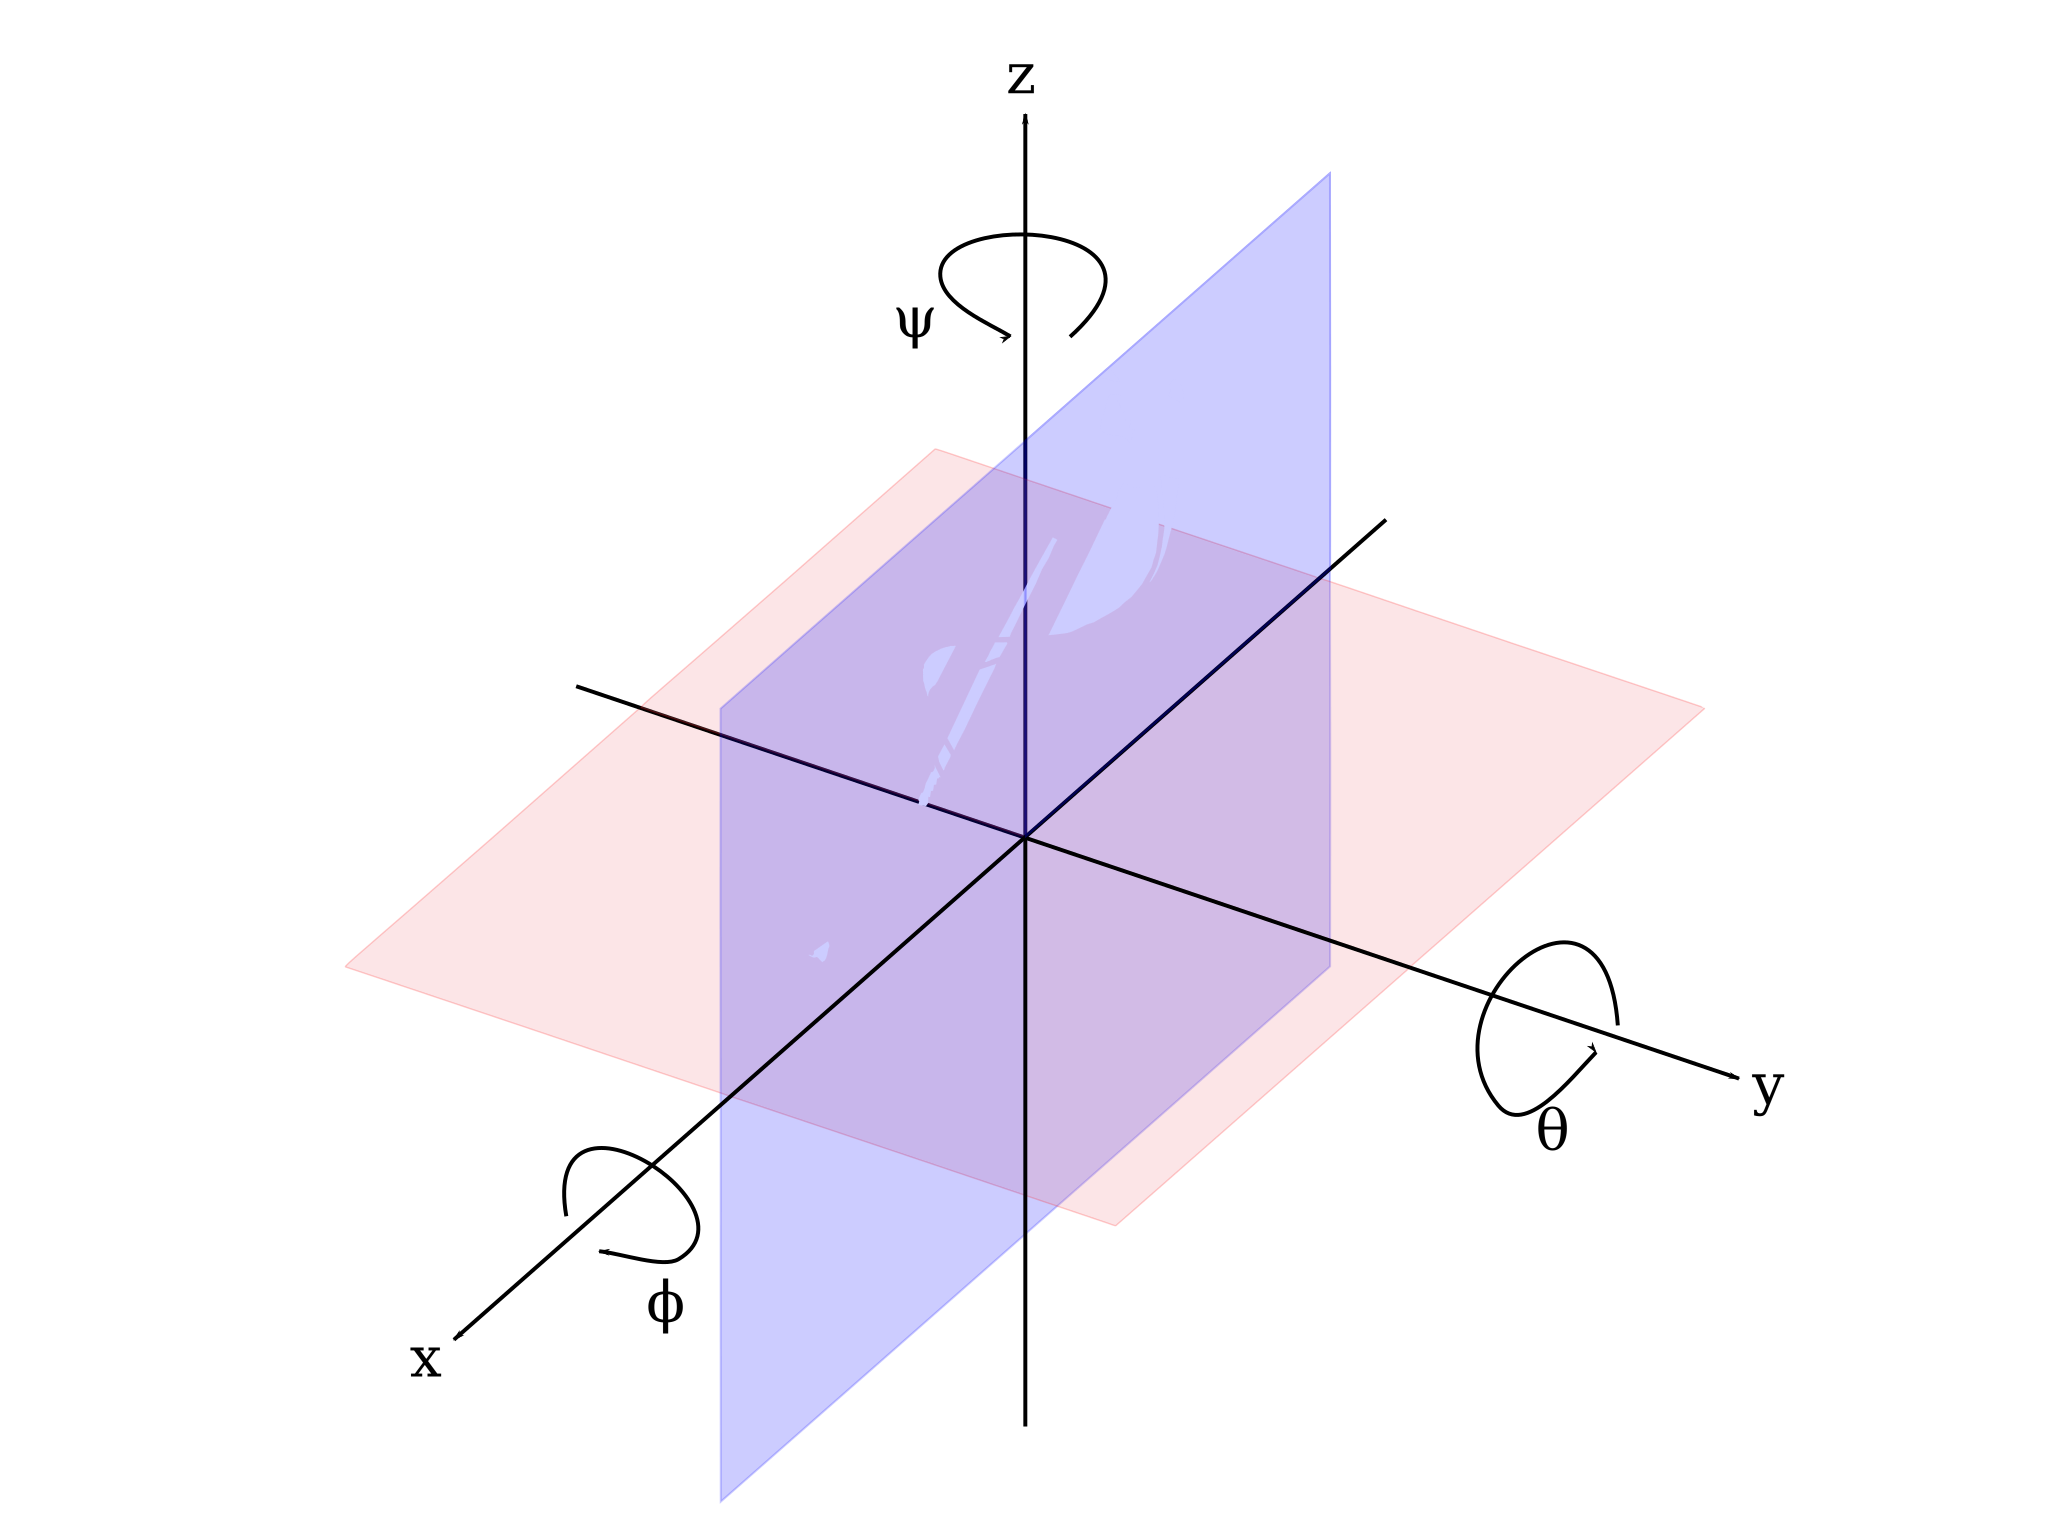
\includegraphics[width=.8\textwidth]{images/packbotaxes}
    \caption{PackBot used in experiments with axes for position and orientation shown.}
    \label{fig:packbotaxes}
\end{figure}

\section{The Kalman Filter}
\label{sec:kalmanfilter}
The ACS Kalman filter is typical of all Kalman filters in that it consists of a prediction update step and a measurement update step where the prediction update is run as fast as possible and the measurement update is run whenever new sensor data becomes available as in Figure \ref{fig:kf}. The prediction update step uses a model of the system dynamics and a measurement of elapsed time to determine where the system is in the world and will inevitably have errors. Some of the errors are due to effects that are not captured in the models, (im)precision of the clock on the computer for measuring time and simplifying assumptions that are made in order to be able to calculate the system model in real-time using embedded computers. The measurement update step is basically a feedback step to help correct for errors in the system model using sensors to provide current data \cite{Kelly_1994_338}.

\begin{figure}[ht!]
	\centering
	\includegraphics[width=.4\textwidth]{images/kf}
	\caption{The Kalman filter algorithm.}
	\label{fig:kf}
\end{figure}

The Kalman filters that run on the small UGVs used in these experiments run on digital computers and are necessarily used in discrete time rather than continuous time because of the nature of computers. Additionally, the standard Kalman filter equations make the assumption that the system and measurement models are linear. From \cite{Kelly_1994_338}, \cite{Simon06OptimalEstimation} the discretized and linearized versions of (\ref{eq:statespace}) mean that the state space equations are represented as
\begin{align*}
%\label{eq:kfstatemodel}
\begin{split}
x_{k+1} &= \Phi_kx_k + w_k \\
y_k &= H_kx_k + v_k
\end{split}
\end{align*}
where $\Phi_k$ is the state transition matrix relating the state at time $k+1$ to time $k$ in the absence of inputs or noise and models the system dynamics, $w_k$ is system noise due to an imperfect model, $H_k$ is the measurement matrix which relates the measurements to the state vector and $v_k$ is the sensor measurement noise. The Kalman filter uses an unforced model so all inputs are considered disturbances to the steady-state dynamics. This means that $w_k$ includes noise, modeling errors, external forces and actuator forces.

The prediction update step marches the system dynamics forward in time using the equations
\begin{align}
\label{eq:kfpredictionupdate}
\begin{split}
\hat{x}_{k+1}^- &= \Phi_k\hat{x}_k^+ \\
P_{k+1}^- &= \Phi_kP_k^+\Phi_k^T + Q_k
\end{split}
\end{align}
and the measurement update step provides feedback from sensor data using the equations
\begin{align}
\label{eq:kfmeasurementupdate}
\begin{split}
K_k &= P_k^-H_k^T\left[H_kP_k^-H_k^T + R_k\right]^{-1} \\
\hat{x}_k^+ &= \hat{x}_k^- + K_k\left[y_k - H_k\hat{x}_k^-\right] \\
P_k^+ &= \left[I - K_kH_k\right]P_k^-.
\end{split}
\end{align}
where $P_k$ is the state covariance matrix, $K_k$ is the Kalman gain, $Q_k$ is the process covariance matrix giving a measure of the expected noise in the system model and $R_k$ is the measurement covariance matrix giving the expected noise of the sensors. Using (\ref{eq:kfpredictionupdate}) and (\ref{eq:kfmeasurementupdate}) an estimate of the state of the robot can be obtained at any time for use by the controls algorithms or to give feedback to a human operator.

The variables $\hat{x}_k^-$ in (\ref{eq:kfpredictionupdate}) and $\hat{x}_k^+$ in (\ref{eq:kfmeasurementupdate}) refer to estimates of the state variables before and after the measurement update step in the Kalman filter, respectively. Each of the terms in the Kalman filter equations is discussed in more detail in subsequent sections.

\subsection{Models in the Kalman Filter}
\label{sec:kfModels}
The Kalman filter relies on several models that are used to determine estimates of the states for a system. The ACS Kalman filter uses four such models:
\begin{itemize}
\item System dynamics model $\Phi$,
\item measurement model $H$,
\item system noise model $Q$,
\item measurement noise model $R$.
\end{itemize}

It is important to recognize that the interaction between these four models determines how well the Kalman filter output will represent the true state of the robot.

\subsection{Assumptions in the System Model}
\label{sec:kfAssumptions}
It is nearly impossible to develop models that completely capture all of the attributes of most systems, including robots that are expected to operate in many different physical environments, so assumptions are made to simplify the system model. The following assumptions allow the prediction update step to be calculated in a reasonable amount of time using modern computers so that a state estimate is available that the control systems can act upon in real time. The assumptions also allow a single system model to be abstracted and used on multiple similar but different robotic vehicles.

\subsubsection{Low Dynamics Assumption}
\label{sec:kfLowDynamicsAssumption}
The first assumption made is that, from one time step to the next, the robot will not be accelerating fast enough in any direction for the sensors on the robot to be able to measure the accelerations. This means that the two velocities, linear and angular, in the state vector will be assumed to be constant. The benefit of this assumption is that there are six fewer states that must be tracked in the state vector, one for acceleration about each axis of the robot.

\subsubsection{Principal Motion Assumption}
\label{sec:kfPrincipalMotionAssumption}
The second assumption says that, during a single time step, the position of the robot will only be a function of linear velocity and the orientation of the robot will only be a function of the angular velocity. Figure \ref{fig:packbotaxes} helps in visualizing the effect of rotating the robot about its center and how that will not affect the position of the robot. Similarly, tranlation of the robot along the $x$ axis will not change the orientation of the robot. This assumption allows several terms in the system model to be set to zero.

\subsection{Continuous to Discrete Time Transform}
\label{sec:kfContToDiscTransform}
The system model will be developed using continuous time nonlinear differential equations but the Kalman filter on the robots will be running on digital computers so the model will need to be converted to discrete time. In continuous time the system model will be
\begin{align*}
\dot{x} = Fx
\end{align*}
and in discrete time the system model will be
\begin{align*}
x_{k+1} = \Phi_k x_k.
\end{align*}
The transformation from continuous to discrete time obeys an exponential matrix transformation with a Taylor series approximation \cite{Gopal93} given by
\begin{align*}
\Phi_k = e^{F\Delta_T} = I + F\Delta_T + \frac{(F\Delta_T)^2}{2!} + \ldots + \frac{(F\Delta_T)^n}{n!}
\end{align*}
A first order Taylor series approximation is good enough when $\Delta_T$ is small and if the nonlinearities in the system are small enough. In the case of the robots used in these experiments that is assumed to be the case so the transformation used is simply
\begin{align}
\label{eq:kfContToDiscTransform}
\Phi_k = I + F\Delta_T.
\end{align}

\subsection{System Dynamics Model}
\label{sec:dynamics}
A model of the system dynamics is necessary in order to propagate the state of the system forward in time in the absence of measurements. It is impossible to create a perfect model of the system and even a nearly perfect model of the system will likely be too complex to compute fast enough for it to be useful. The best result that is typically available is a model with a large amount of assumptions where the most important aspects of the dynamics are captured in the model.

A nonlinear, continuous time model based on robot kinematics is developed in the body frame coordinate system using the states from section \ref{sec:statespacemodels} is given by
\begin{align}
\label{eq:kfnonlineardynamics}
\begin{split}
\frac{d}{dt}\left[\begin{array}{c}
x \\ y \\ z \\ V \\ \theta \\ \phi \\ \psi \\ \omega
\end{array}\right] =
\left[\begin{array}{c}
V\cos\psi\cos\theta \\
V\sin\psi\cos\theta \\
-V\sin\theta \\
0 \\
-\omega\sin\phi \\
\omega\tan\theta\cos\phi \\
\omega\cos\phi/\cos\theta \\
0
\end{array}\right].
\end{split}
\end{align}

\subsection{Extended Kalman Filter}
\label{sec:extendedkf}
The basic Kalman filter makes the assumption that both the system model contained in $\Phi_k$ and the measurement model in $H_k$ are linear. The extended Kalman filter (EKF) allows for nonlinear models such as that given by (\ref{eq:kfnonlineardynamics}) to be used for $\Phi_k$, $H_k$ or both by linearizing the models around the state estimate. To linearize the models the Jacobian, or matrix of partial derivatives, is taken about the estimated state. The idea of linearization of a nonlinear model is shown in Figure \ref{fig:KFLinearization} where the linearization can be seen to be more accurate when the system nonlinearities are small meaning that the dynamics are slow.

\begin{figure}[ht!]
	\centering
    \subfloat[Slow dynamics.] {
	    \label{images/KFLinearizationSlow}
        \includegraphics[width=.3\textwidth]{images/KFLinearizationSlow}
    }
    \hfill
    \subfloat[Medium dynamics.] {
        \label{images/KFLinearizationMedium}
	    \includegraphics[width=.3\textwidth]{images/KFLinearizationMedium}
    }
    \hfill
    \subfloat[Fast dynamics.] {
        \label{images/KFLinearizationFast}
	    \includegraphics[width=.3\textwidth]{images/KFLinearizationFast}
    }
	\caption{Effects of linearizing a nonlinear model. Success depends on the speed of the dynamics, either \subref{images/KFLinearizationSlow} slow, \subref{images/KFLinearizationMedium} medium or \subref{images/KFLinearizationFast} fast.}
	\label{fig:KFLinearization}
\end{figure}

The nonlinear state dynamics were described in (\ref{eq:kfnonlineardynamics}). The Jacobian of that state vector equation is calculated using
%{\tiny
\begin{align*}
\frac{d}{dt}\left[\begin{array}{c}
x \\ y \\ z \\ V \\ \theta \\ \phi \\ \psi \\ \omega
\end{array}\right] =
\underbrace{\left[\begin{array}{c c c c c c c c}
\frac{\partial \dot{x}}{\partial x} & \frac{\partial \dot{x}}{\partial y} & \frac{\partial \dot{x}}{\partial z} & \frac{\partial \dot{x}}{\partial V} & \frac{\partial \dot{x}}{\partial \theta} & \frac{\partial \dot{x}}{\partial \phi} & \frac{\partial \dot{x}}{\partial \psi} & \frac{\partial \dot{x}}{\partial \omega} \\
\frac{\partial \dot{y}}{\partial x} & \frac{\partial \dot{y}}{\partial y} & \frac{\partial \dot{y}}{\partial z} & \frac{\partial \dot{y}}{\partial V} & \frac{\partial \dot{y}}{\partial \theta} & \frac{\partial \dot{y}}{\partial \phi} & \frac{\partial \dot{y}}{\partial \psi} & \frac{\partial \dot{y}}{\partial \omega} \\
\frac{\partial \dot{z}}{\partial x} & \frac{\partial \dot{z}}{\partial y} & \frac{\partial \dot{z}}{\partial z} & \frac{\partial \dot{z}}{\partial V} & \frac{\partial \dot{z}}{\partial \theta} & \frac{\partial \dot{z}}{\partial \phi} & \frac{\partial \dot{z}}{\partial \psi} & \frac{\partial \dot{z}}{\partial \omega} \\
\frac{\partial \dot{V}}{\partial x} & \frac{\partial \dot{V}}{\partial y} & \frac{\partial \dot{V}}{\partial z} & \frac{\partial \dot{V}}{\partial V} & \frac{\partial \dot{V}}{\partial \theta} & \frac{\partial \dot{V}}{\partial \phi} & \frac{\partial \dot{V}}{\partial \psi} & \frac{\partial \dot{V}}{\partial \omega} \\
\frac{\partial \dot{\theta}}{\partial x} & \frac{\partial \dot{\theta}}{\partial y} & \frac{\partial \dot{\theta}}{\partial z} & \frac{\partial \dot{\theta}}{\partial V} & \frac{\partial \dot{\theta}}{\partial \theta} & \frac{\partial \dot{\theta}}{\partial \phi} & \frac{\partial \dot{\theta}}{\partial \psi} & \frac{\partial \dot{\theta}}{\partial \omega} \\
\frac{\partial \dot{\phi}}{\partial x} & \frac{\partial \dot{\phi}}{\partial y} & \frac{\partial \dot{\phi}}{\partial z} & \frac{\partial \dot{\phi}}{\partial V} & \frac{\partial \dot{\phi}}{\partial \theta} & \frac{\partial \dot{\phi}}{\partial \phi} & \frac{\partial \dot{\phi}}{\partial \psi} & \frac{\partial \dot{\phi}}{\partial \omega} \\
\frac{\partial \dot{\psi}}{\partial x} & \frac{\partial \dot{\psi}}{\partial y} & \frac{\partial \dot{\psi}}{\partial z} & \frac{\partial \dot{\psi}}{\partial V} & \frac{\partial \dot{\psi}}{\partial \theta} & \frac{\partial \dot{\psi}}{\partial \phi} & \frac{\partial \dot{\psi}}{\partial \psi} & \frac{\partial \dot{\psi}}{\partial \omega} \\
\frac{\partial \dot{\omega}}{\partial x} & \frac{\partial \dot{\omega}}{\partial y} & \frac{\partial \dot{\omega}}{\partial z} & \frac{\partial \dot{\omega}}{\partial V} & \frac{\partial \dot{\omega}}{\partial \theta} & \frac{\partial \dot{\omega}}{\partial \phi} & \frac{\partial \dot{\omega}}{\partial \psi} & \frac{\partial \dot{\omega}}{\partial \omega}
\end{array}\right]}_{F}
\left[\begin{array}{c}
x \\ y \\ z \\ V \\ \theta \\ \phi \\ \psi \\ \omega
\end{array}\right]
\end{align*}
%}
which results in
%{\scriptsize
{\footnotesize
\begin{align}
\label{eq:kfjacobianresult}
\frac{d}{dt}\left[\begin{array}{c}
x \\ y \\ z \\ V \\ \theta \\ \phi \\ \psi \\ \omega
\end{array}\right] =
\underbrace{\left[\begin{array}{c c c c c c c c}
0 & 0 & 0 & c\psi c\theta & -V c\psi s\theta               & 0                     & -V s\psi c\theta & 0 \\
0 & 0 & 0 & s\psi c\theta & -V s\psi s\theta               & 0                     & V c\psi c\theta  & 0 \\
0 & 0 & 0 & -s\theta      & -V c\theta                     & 0                     & 0                & 0 \\
0 & 0 & 0 & 0             & 0                              & 0                     & 0                & 0 \\
0 & 0 & 0 & 0             & 0                              & -\omega c\phi         & 0                & -s\phi \\
0 & 0 & 0 & 0             & \omega c\phi/c^2\theta         & \omega t\theta s\phi  & 0                & t\theta c\phi \\
0 & 0 & 0 & 0             & \omega s\theta c\phi/c^2\theta & -\omega s\phi/c\theta & 0                & c\phi/c\theta \\
0 & 0 & 0 & 0             & 0                              & 0                     & 0                & 0
\end{array}\right]}_{F}
\left[\begin{array}{c}
x \\ y \\ z \\ V \\ \theta \\ \phi \\ \psi \\ \omega
\end{array}\right].
\end{align}
}
Applying the principal motion assumption to set the terms relating position and angular velocity as well as orientation and linear velocity to zero in addition to converting from continuous to discrete time to put ones on the diagonal (c.f. (\ref{eq:kfContToDiscTransform})) gives
\begin{align*}
%\label{eq:kfSystemModelWithAssumptions}
x_{k+1} = 
\underbrace{\left[\begin{array}{c c c c c c c c}
1 & 0 & 0 & c\psi c\theta \Delta_T & 0 & 0 & 0 & 0 \\
0 & 1 & 0 & s\psi c\theta \Delta_T & 0 & 0 & 0 & 0\\
0 & 0 & 1 & -s\theta \Delta_T & 0 & 0 & 0 & 0\\
0 & 0 & 0 & 1 & 0 & 0 & 0 & 0 \\
0 & 0 & 0 & 0 & 1 & 0 & 0 & -s\phi \Delta_T \\
0 & 0 & 0 & 0 & 0 & 1 & 0 & t\theta c\phi \Delta_T \\
0 & 0 & 0 & 0 & 0 & 0 & 1 & c\phi \Delta_T/c\theta \\
0 & 0 & 0 & 0 & 0 & 0 & 0 & 1
\end{array}\right]}_{\Phi_k}
\left[\begin{array}{c}
x \\ y \\ z \\ V \\ \theta \\ \phi \\ \psi \\ \omega
\end{array}\right]_k
\end{align*}
as the system model that is used in the prediction update step of the Kalman filter equations to calculate the state of the robot in between measurements.

\subsection{Measurement Model}
\label{sec:kfMeasurementModel}
The measurement model converts sensor data to the state variable coordinate system and for a standard sensor suite is by far the simplest model used in the ACS Kalman filter. The idea is that, for a sensor that measures one of the states, the data that is output by the sensor has to have the same units and be in the same range as the state variable. This is best illustrated by an example.

Suppose a compass and an IMU both measure the yaw state variable and the compass output is $0 - 360^\circ$ whereas the IMU output is $0 - 2\pi~rads$ and the yaw state in the Kalman filter is tracked in the range $0 - 2\pi ~ rads$. If, for one time step, both compass and IMU measurements are available to be incorporated into the Kalman filter then the measurement update step from (\ref{eq:kfmeasurementupdate}) is run and the $H$ matrix is
\begin{align*}
H = \left[\begin{array}{c c c c c c c c}
0 & 0 & 0 & 0 & 0 & 0 & \frac{\pi}{180^\circ} & 0 \\
0 & 0 & 0 & 0 & 0 & 0 & 1 & 0
\end{array}\right]
\end{align*}
and the $y$ vector is a $2\times1$ column vector with the compass measurement in the $y_{(1,1)}$ element and the IMU measurement in the $y_{(2,1)}$ element.

There is one row per sensor measurement and one column per state in the measurement matrix so in this example $H$ is a $2\times8$ matrix. The compass measurement corresponds to the first row and the data is converted from degrees to radians. The IMU measurement corresponds to the second row and, since the units of the sensor data are the same as the units of the state variable, the data is not transformed at all.

In the case when there is a single sensor measuring each of the states and those sensors output data that is in the correct units and range of the state variables then $H=I$.

\subsection{Noise Models}
\label{sec:kfNoiseModels}
The noise models attempt to estimate noise coming in from the terms in the equations
\begin{align*}
\begin{split}
x_{k+1} &= \Phi_kx_k + w_k \\
y_k &= H_kx_k + v_k.
\end{split}
\end{align*}

The Kalman filter uses two different noise models, one for system noise $w_k$ and one for measurement noise $v_k$. The system noise model attempts to capture all of the effects due to an imperfect system model, linearization of the model, the low dynamics assumption and the principal motion assumption. The measurement noise model tries to compensate for sensors that do not model the environment perfectly.

Noise in the Kalman filter is assumed to be zero mean with a Gaussian distribution. The models are set up as covariance matrices that describe the Gaussian distribution of each of the noise terms for either the states or the sensors where the state noise model is given by $Q$ and the measurement noise model is given by $R$. When the noise in the system is \textit{not} Gaussian then the Kalman filter is the best linear estimator and performance will degrade gracefully as non-Gaussian noise enters the system \cite{Simon10}. As noted in \cite{AndersonMoore79} when dropping the Gaussian assumption all of the Kalman filter equations will propagate exactly the same for the mean and covariance of the states and measurements except that any information about higher order moments is lost and the probability density functions cannot be reproduced. This means that the Gaussian assumption is valid when the higher order moments do not have a large effect on the noise distributions. When the higher order moments are significant then the Kalman filter performance will degrade gracefully and still be the optimal linear filter.

\subsection{Kalman Gain}
\label{kfKalmanGain}
The Kalman gain matrix is used in the measurement update step (\ref{eq:kfmeasurementupdate}) and essentially weights whether the state estimate will rely more on the system model or the measurements and is given by
\begin{align*}
K_k &= P_k^-H_k^T\left[H_kP_k^-H_k^T + R_k\right]^{-1}
\end{align*}
where
\begin{align*}
P_{k+1}^- &= \Phi_kP_k^+\Phi_k^T + Q_k.
\end{align*}

From these equations it can be seen that all four models used in the Kalman filter are used to calculate the Kalman gain matrix since $\Phi$, $Q$, $H$ and $R$ are all present. In the measurement update step the Kalman gain is multiplied by the difference between the measured values $y_k$ of the state and the expected values of those measurements based on the system model $\hat{y}_k$ where $\hat{y}_k = H\hat{x}_k^-$ is what the sensors would report if there were no noise in the measurements and the system model were perfect. The state estimate from the measurement update step is
\begin{align*}
\hat{x}_k^+ &= \hat{x}_k^- + K_k\left[y_k - H_k\hat{x}_k^-\right].
\end{align*}

If the sensor data matches the system model prediction then the innovations term $y_k-H_k\hat{x}_k^-=0$ and the Kalman gain is ignored but that rarely, if ever, happens in practice. The interesting question then becomes whether to trust the noisy sensors or the imperfect system model to determine the state estimate. A large gain value will adjust the previous estimate from the prediction update step by a larger amount which means that the sensor data is weighted more heavily than the system model. Conversely a small gain value will cause the estimate from the measurement update step to trust the system model more than the sensor data. It is important to note that the Kalman gain matrix $K$ can have large values for some states (and sensors) and small values for other states (and sensors).

As discussed in section \ref{sec:kfMeasurementModel} the measurement model is fairly simple so the Kalman gain is really a function of the system model and the noise models. If the system model is a very good approximation to the real system then the system noise model should reflect that by having small values in $Q$ and if the sensors are very good then the measurement noise model will have small values in $R$. Thus the Kalman gain matrix tends to take on values relative to the ratio of the elements of the $Q$ and $R$ noise models. From this it can be seen that developing accurate noise models is very important to the performance of the Kalman filter.

When the models are not set up correctly then the measurements will likely not match the predicted state estimates and the Kalman gains will grow larger during each measurement update step to force the state estimate to trust the measurements more than the system model.

\section{Determining Heading}
\label{sec:determineHeading}
An immediate problem that arose during testing which had to be addressed before new techniques such as those in section \ref{sec:kftrainingparams} and \ref{sec:controllyapunov} could be attempted is that the robots did not always know which direction they were heading due to a lack of sensors. The original sensors used to determine heading on the robots were GPS and a gyro in the IMU. GPS worked fine when the robot was driving forward but when the robot began to drive in reverse the heading would rotate $180^\circ$. The angular velocity measurement from the gyro was integrated over time using the system model from (\ref{eq:kfjacobianresult}) and included as a second heading measurement although this measurement tends to drift over longer periods. An Ocean Server OS5000 digital compass was added to get a better estimate of heading in a global coordinate system since the magnetometer performance was better with that sensor than with the Microstrain 3DM-GX1 and wheel encoder measurements of linear and angular velocity were also added. The velocities from the encoders were directly incorporated into the measurement update step and the sign of the linear velocity was used to determine the appropriate to use for GPS heading.

Figure \ref{fig:GEHeadingReverse} shows the routes driven by the robot when testing heading where the heading was reversed on the blue route and the heading was fixed on the red route. Figure \ref{fig:pbDataReverseHeadingBroken} shows sensor data before adding the encoder data to the Kalman filter (but using logged encoder data for comparison purposes to show where the velocity was negative) and the heading can be seen to flip $\pi ~ rads$ where the velocity was negative but the GPS velocity is positive. Figure \ref{fig:pbDataReverseHeadingFixed} is the sensor data after incorporating the encoder velocities into the Kalman filter and using the encoder data to reverse the sign of the GPS velocity whenever the encoder velocity is negative which results in a heading estimate that does not flip.

\begin{figure}[ht!]
	\centering
	\includegraphics[width=.7\textwidth]{images/GEHeadingReverseFixed}
	\caption{Route Driven by PackBot}
	\label{fig:GEHeadingReverse}
\end{figure}

\begin{figure}[ht!]
	\centering
	\includegraphics[width=.7\textwidth]{images/pbDataReverseHeading}
	\caption{Heading and Velocity Reversed}
	\label{fig:pbDataReverseHeadingBroken}
\end{figure}

\begin{figure}[ht!]
	\centering
	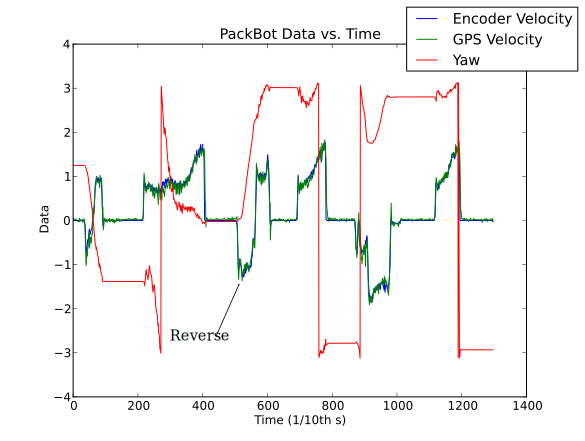
\includegraphics[width=.7\textwidth]{images/KFDataHeadingReverseFixed}
	\caption{Heading Fixed When Driving in Reverse}
	\label{fig:pbDataReverseHeadingFixed}
\end{figure}

Adding the Ocean Server OS5000 digital compass allowed the variance of the Mictrostrain 3DM-GX1 angular rate sensor to be set much higher than the original variance and led to a more accurate heading estimate. Figure \ref{fig:pbDataLowYRVar} shows data captured while the robot was spinning in place and it can be seen that the compass yaw and Kalman filter heading estimate do not match very well. When the variance of the gyro data was greatly increased the Kalman filter heading estimate began to track the compass heading output very closely as seen in Figure \ref{fig:pbDataHighYRVar}.

\begin{figure}[ht!]
	\centering
	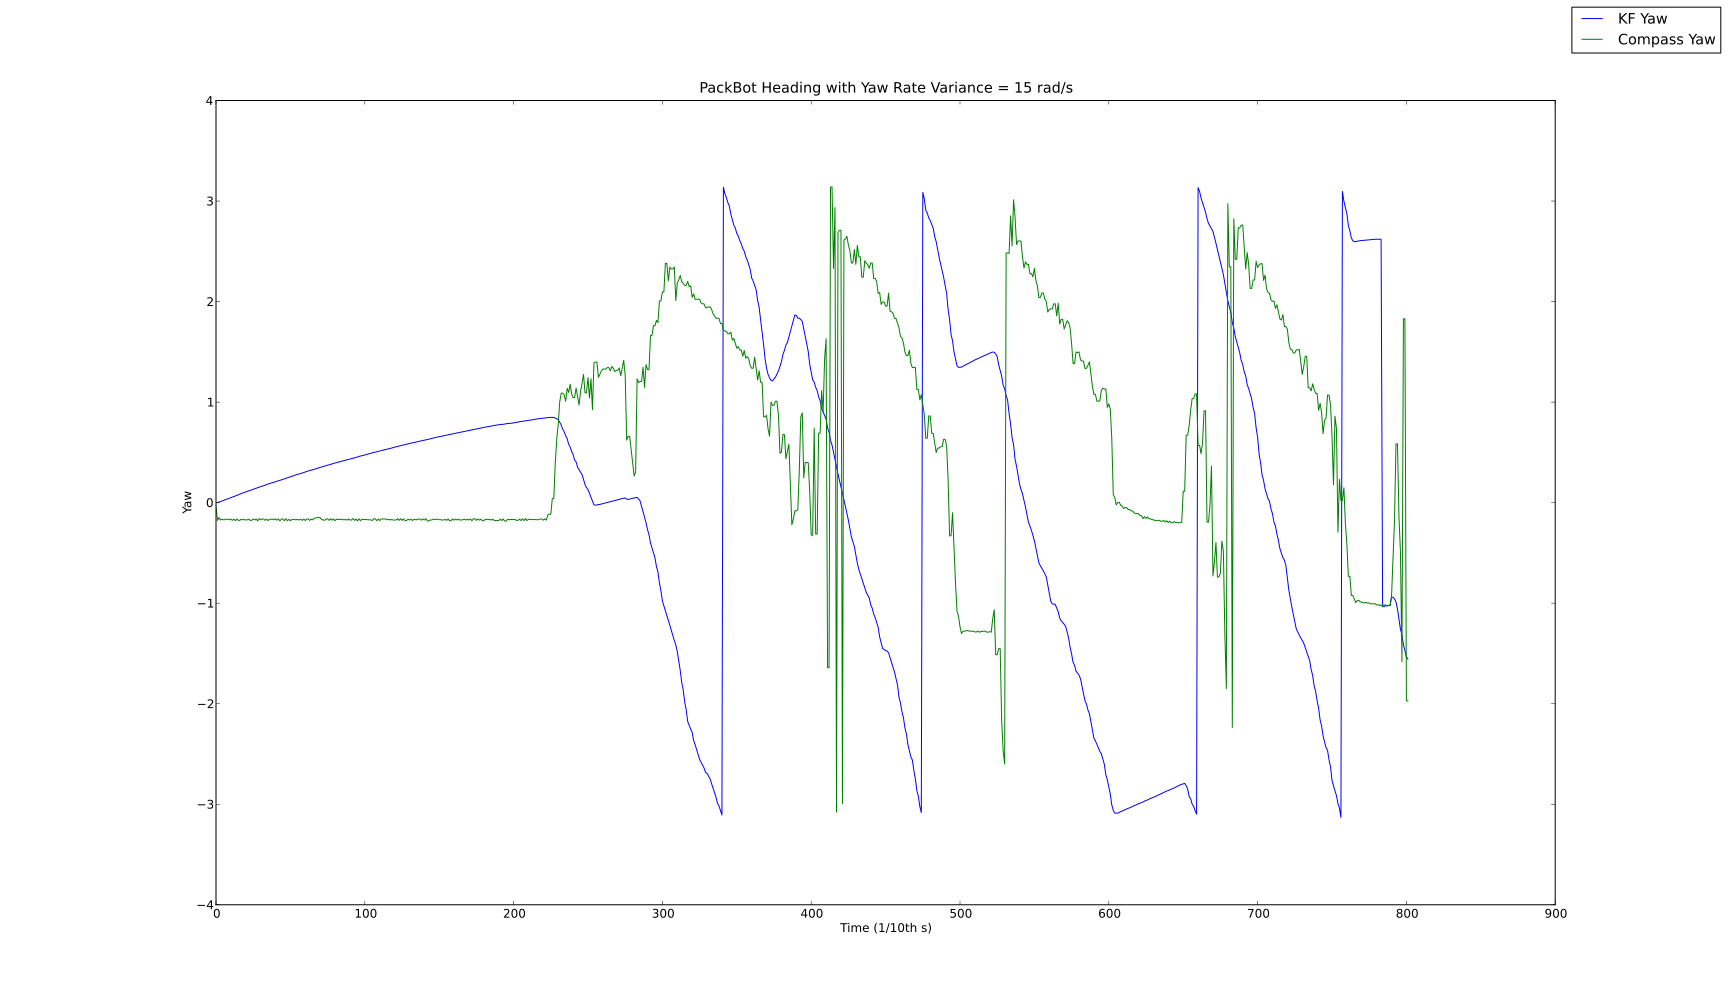
\includegraphics[width=.8\textwidth]{images/pbDataLowYRVar}
	\caption{Low Variance for Yaw Rate Sensor}
	\label{fig:pbDataLowYRVar}
\end{figure}

\begin{figure}[ht!]
	\centering
	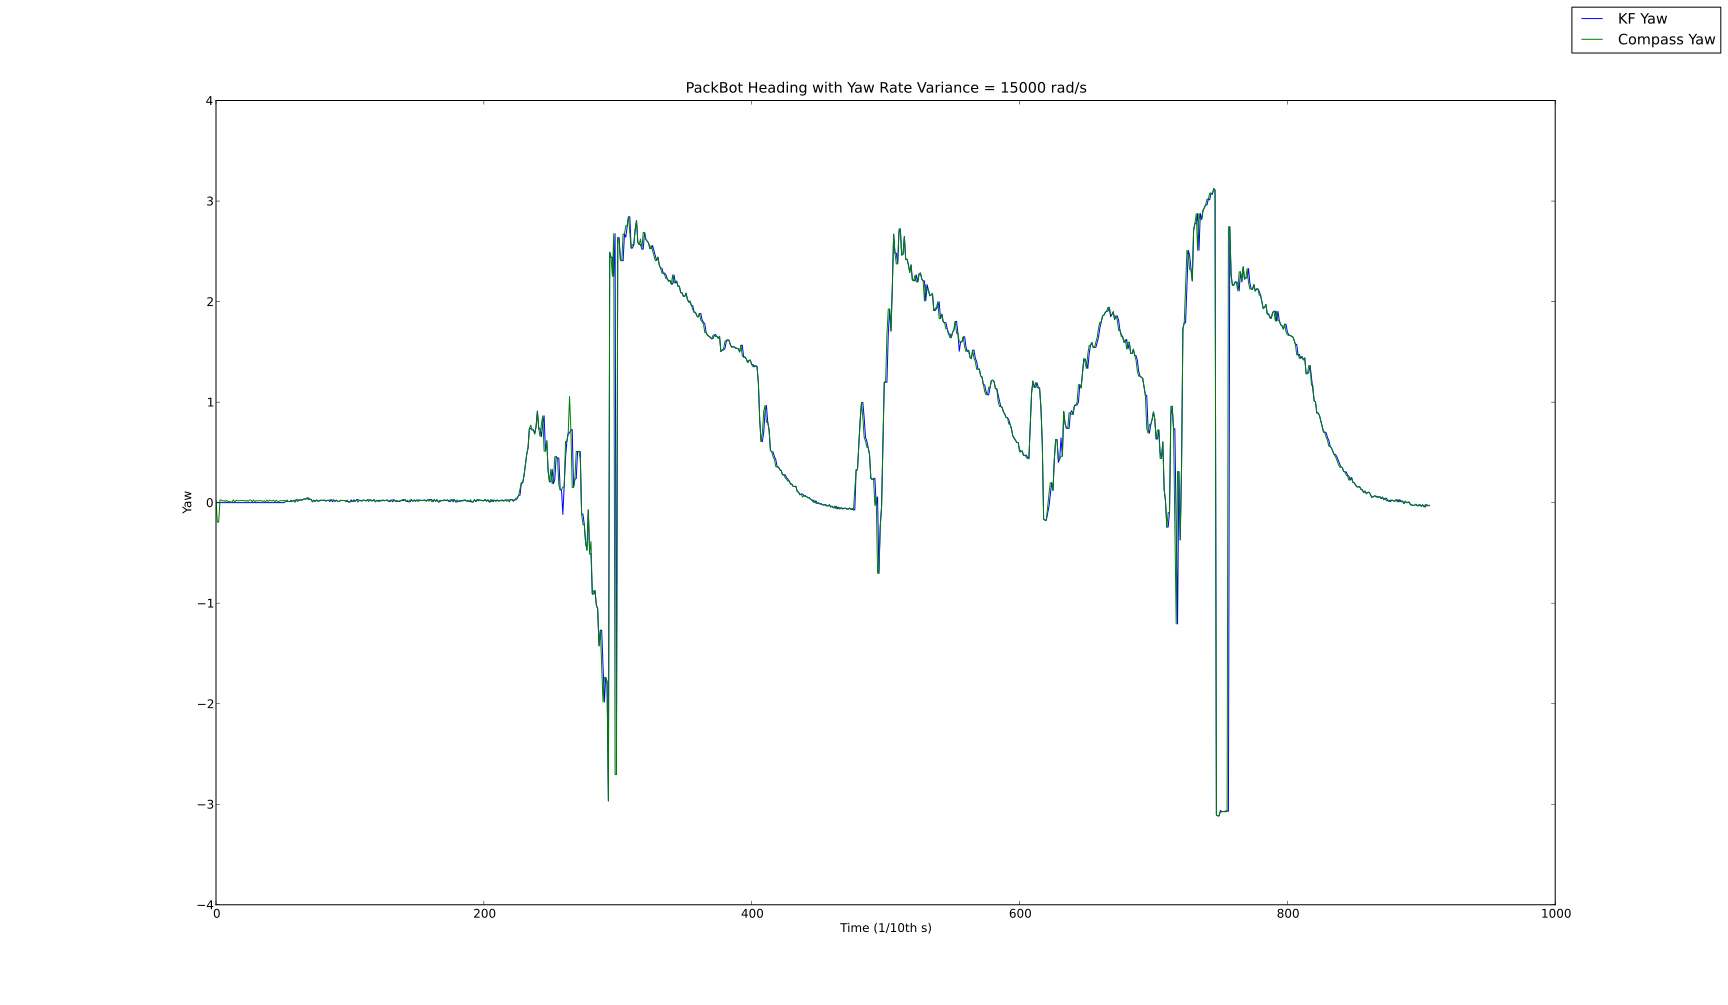
\includegraphics[width=.8\textwidth]{images/pbDataHighYRVar}
	\caption{High Variance for Yaw Rate Sensor}
	\label{fig:pbDataHighYRVar}
\end{figure}

\section{Establishing Ground Truth}
\label{sec:groundtruth}
Quantitatively evaluating the performance of Kalman filters can be accomplished in several ways, the best of which is to analyze the output of the Kalman filter against ground truth. Although it is nearly impossible to establish ground truth over a large area in practice the closer the measurements are to an absolute position in the world the better. To determine ground truth for the robots in these experiments a differential GPS (DGPS) system was created independently of the sensors on the robot so that very accurate measurements of the robots actual position could be logged and then used in a post-processing step to determine how well the Kalman filter estimate corresponds to ground truth.

The DGPS system consists of a GPS receiver and serial radio that make up the base station and a GPS receiver, serial radio and small computer that make up the roaming station as in Figure \ref{fig:dgps}. The GPS receivers are both Novatel receivers using the Real Time Kinematics algorithm. The base station is located in a static position and is configured to use a fixed position which is compared to what the current position would be if it were not fixed. The difference between the fixed position and the calculated position are used to generate corrections that would put the position of the GPS antenna at the fixed position and those corrections are sent to and applied at the roaming station resulting in a standard deviation of $2$ $cm$ for the position output of the roaming station. The errors are due to the effects of the GPS signal passing through the atmosphere from the satellites to the antenna as well as to multipath effects closer to the ground. The DGPS corrections are used for each satellite that the ground station and the roaming station share in the constellation of satellites they are using in their solution of a position estimate. The DGPS system is bootstrapped to the robot during testing runs to log data at a rate of $20$ $Hz$ and is only used as a tool to improve Kalman filter performance and is not meant to be used during normal operation.

With a highly accurate estimate of ground truth established it becomes possible to not only study the performance of the Kalman filter but to also begin determining whether to focus efforts in improving the autonomous navigation behaviors of the robots via the estimation or controls algorithms.

\begin{figure}[ht!]
	\centering
	\includegraphics[width=.6\textwidth]{images/dgps}
	\caption{Differential GPS system diagram.}
	\label{fig:dgps}
\end{figure}

\section{Identifying Noise Models}
\label{sec:kfIdentifyNoiseModels}
Attempting to determine the proper values for the noise models $Q$ in (\ref{eq:kfpredictionupdate}) and $R$ in (\ref{eq:kfmeasurementupdate}) can be a laborious process and is often considered more of an art than a science with engineer experience being a critical factor. In section \ref{sec:kfNoiseModels} it was shown that the Kalman filter performance is heavily dependent upon the accuracy of the noise models even though they are difficult to determine. Several complementary methods exist to assist engineers in determining proper relative weighting of the elements in $Q$ and $R$ to improve Kalman filter performance after initial values are selected by the engineer.

\subsection{Adaptive Extended Kalman Filter}
\label{sec:adaptiveekf}
*** Why is it valid to update $Q$ and $R$ this way? Talk about how the updates are turned off when the velocity is zero, otherwise $Q$ and $R$ are adapted to a static, not dynamic, state. Similarly, talk about how this method doesn't work as well as would be hoped because the original application was for tracking satellites with low dynamics and robots have high dynamics, especially when navigating around obstacles. Also, look at the extra stuff that Busse says he had to do to get this algorithm to work in practice. I say high dynamics here, but what about the low dynamics assumption? Low is relative to sensor noise and satellites have much higher quality sensors so the noise level is much lower in addition to the actual dynamics being lower. ***

In order to improve the noise models the ACS Kalman filter has been implemented with an adaptive scheme to update the covariance matrices $Q$ and $R$ in real time as the robot moves around and sensor measurements are taken into account to help overcome the time intensive nature of determining these matrices and add a degree of robustness to the state estimate \cite{Sights06}, \cite{Mehra72}, \cite{Busse03adaptiveEKF}. Estimates of $Q$ and $R$ are updated at alternating time steps in the EKF. Recall from (\ref{eq:kfpredictionupdate}) and (\ref{eq:kfmeasurementupdate}) that $\hat{x}_k^+$ and $P_k^+$ are known after the measurement update step and $\hat{x}_k^-$ and $P_k^-$ are known after the system update step in the Kalman filter.

As shown in \cite{Busse03adaptiveEKF} the first step is to calculate $Q^\star$ using
\begin{align*}
% \label{eq:qstar}
Q^\star = \left(\hat{x}_k^+-\hat{x}_k^-\right)\left(\hat{x}_k^+-\hat{x}_k^-\right)^T + P_k^- - P_k^+ - \hat{Q}_k^-.
\end{align*}
Then the estimate of $Q$ is updated such that
\begin{align}
\label{eq:qadapt}
\hat{Q}_k^+ = \hat{Q}_k^- + \frac{1}{L_Q}\left(Q^\star-\hat{Q}_k^-\right).
\end{align}

Next $R^\star$ is calculated using
\begin{align*}
% \label{eq:rstar}
R^\star = \left(y_k-\hat{y}_k^+\right)\left(y_k-\hat{y}_k^+\right)^T - H_kP_k^+H_k^T
\end{align*}
where $y_k$ are actual measurement data and $\hat{y}_k^+ = h_k\hat{x}_k^+$ is calculated after the measurement update step. Then the estimate of $R$ is updated such that
\begin{align}
\label{eq:radapt}
\hat{R}_k^+ = \hat{R}_k^- + \frac{1}{L_R}\left(R^\star-\hat{R}_k^-\right).
\end{align}
It can be seen that the estimates of both covariance matrices employ a running average algorithm and vary the weight of recent measurements and state updates via the adaptation coefficients $L_Q$ and $L_R$.

\subsection{Discriminative Training of Kalman Filter Parameters}
\label{sec:kftrainingparams}
*** Investigate the difference between adaptive filtering and training. It seems like they accomplish the same thing, namely, convergence to some values for the covariance matrices. Do they use the same metrics? Do they converge to the same covariance matrices? Is it just online vs. offline training? Would a neural network be a good candidate for finding $Q$ and $R$ as well? All of these methods seem to be curve fitting in the multi-dimensional state space. Look at \S3.3 of \cite{Simon06OptimalEstimation} for details on how measurements affect state estimate via recursive least squares. I might also use \cite{Orderud05}. ***

\cite{Abbeel-RSS-05} describes a method to automatically learn what the covariance matrices $Q$ and $R$ should be that is an alternative, offline approach to the adaptive EKF from section \ref{sec:adaptiveekf}. However, when used in conjunction with the adaptive EKF scheme this could allow for faster convergence times when the robots are started and for smaller ranges for the adaptation coefficients $L_Q$ and $L_R$ in (\ref{eq:qadapt}) and (\ref{eq:radapt}). This method takes advantage of ground truth measurements obtained using a DGPS system like that described in section \ref{sec:groundtruth}. Note that in the following expressions the term $h(\mu_t)$ is the position output by the Kalman filter and $y$ is the DGPS position output so the goal is to find values of $Q$ and $R$ that minimizes the difference between the output of the Kalman filter and DGPS ground truth.

There are several metrics that can be applied to the data with the two most relevant metrics being the residual error metric and the prediction likelihood error metric. The residual prediction error is used to estimate $Q$ and $R$ using
\begin{align*}
\left<R_{\text{res}},Q_{\text{res}}\right> = \argmin_{R,Q}\sum_{t=0}^T ||y_t-h(\mu_t)||_2^2.
\end{align*}
When the state covariance matrix $P$ is \textit{not} a multiple of the identity matrix $I$ then this metric is
\begin{align*}
\left<R_{\text{res}},Q_{\text{res}}\right> = \argmin_{R,Q}\sum_{t=0}^T (y_t-h(\mu_t))^TP^{-1}(y_t-h(\mu_t)).
\end{align*}
The error metric used for the residual prediction error method is
\begin{align}
\label{eq:kftrainingres}
e = \left(\frac{1}{T}\sum_{t=1}^T ||h(\mu_t)-y_t||^2\right)^{1/2}.
\end{align}

The prediction likelihood method use the metric
\begin{align*}
\left<R_{\text{pred}},Q_{\text{pred}}\right> = \argmax_{R,Q}\sum_{t=0}^T -\log|2\pi\Omega_t| - (y_t-h(\mu_t))^T\Omega_t^{-1}(y_t-h(\mu_t))
\end{align*}
where $\Omega = H_t\Sigma_tH_t^T+P$. The error metric used for the prediction likelihood method is
\begin{align}
\label{eq:kftrainingpred}
e = -\frac{1}{T}\sum_{t=1}^T \left(\log|2\pi\Omega_t| - (y_t-h(\mu_t))^T\Omega_t^{-1}(y_t-h(\mu_t))\right)
\end{align}
where $\Omega$ is the same as in the above description.

A program was written to implement these algorithms where logged data -- both from the output of the Kalman filter running on the robot and ground truth as recorded from the DGPS system -- is used to try all the possible combinations of $Q$ and $R$ matrices until the metrics identified in (\ref{eq:kftrainingres}) and (\ref{eq:kftrainingpred}) are minimized or maximized to within some convergence criterion. This method of searching is called \textit{coordinate descent}. The possible $Q$ and $R$ matrices start with a coarse grid and are reduced to a finer grid at each iteration where the grid is centered around the best estimate found from the previous grid.

\subsection{Numerical Analysis of Training Program}
\label{sec:trainingNumericalAnalysis}
The training program used here is a brute-force coordinate descent approach to finding the optimal $Q$ and $R$ matrices for the Kalman filter. The number of matrices attempted can grow to a very large number when all elements of the matrices are varied so an optional algorithm was developed that trains using only diagonal $Q$ and $R$ matrices. This is not an unreasonable restriction as the original $Q$ and $R$ matrices found by hand-tuning or from the output of the adaptive Kalman filter from section \ref{sec:adaptiveekf} used only diagonal $Q$ and $R$ matrices. The number of possible matrices that are used during training is a function of the number of states used in the Kalman filter and the number of measurements where
\begin{align*}
%\label{eq:trainingFullMatrices}
\begin{split}
n_Q &= 3^{n_{states}^2} \\
n_R &= 3^{n_{measurements}^2} \\
% n_Q &= 2^{n_{states}^2} \\
% n_R &= 2^{n_{measurements}^2} \\
n_{full} &= n_Q \times n_R
\end{split}
\end{align*}
for varying all elements of $Q$ and $R$ and
\begin{align*}
%\label{eq:trainingDiagonalMatrices}
\begin{split}
% n_Q &= 2^{n_{states}} \\
% n_R &= 2^{n_{measurements}} \\
n_Q &= 3^{n_{states}} \\
n_R &= 3^{n_{measurements}} \\
n_{diagonal} &= n_Q \times n_R
\end{split}
\end{align*}
for varying only the diagonal elements of $Q$ and $R$. During the experiments conducted the number of states is $8$ and the number of measurements is $5$ which gives
\begin{align*}
\begin{split}
% n_Q &= 2^{8^2} = 18446744073709551616 \\
% n_R &= 2^{5^2} = 33554432 \\
n_Q &= 3^{8^2} = 3433683820292512484657849089281 \\
n_R &= 3^{5^2} = 847288609443 \\
n_{full} &= n_Q \times n_R \\
% &= 618970019642690137449562112
&= 2909321189362570808630465826492242446680483
\end{split}
\end{align*}
per grid level when varying all elements of $Q$ and $R$ and
\begin{align*}
\begin{split}
% n_Q &= 2^8 = 256 \\
% n_R &= 2^5 = 25 \\
n_Q &= 3^8 = 6561 \\
n_R &= 3^5 = 243 \\
% n_{diagonal} &= n_Q \times n_R = 6400
n_{diagonal} &= n_Q \times n_R = 1594323
\end{split}
\end{align*}
per grid level when varying only the diagonal elements of $Q$ and $R$. The ratio is
\begin{align*}
%\label{eq:trainingRatio}
\begin{split}
r &= \frac{n_{full}}{n_{diagonal}} \\
% &= \frac{2^{n_{states}^2} \times 2^{n_{measurements}^2}}{2^{n_{states}} \times 2^{n_{measurements}}} \\
% &= 2^{n_{states}} \times 2^{n_{measurements}} \\
% &= 2^8 \times 2^5 = 8192
&= \frac{3^{n_{states}^2} \times 3^{n_{measurements}^2}}{3^{n_{states}} \times 3^{n_{measurements}}} \\
&= 3^{n_{states}} \times 3^{n_{measurements}} \\
&= 3^8 \times 3^5 = 1594323
\end{split}
\end{align*}
which means that it will take $1,594,323$ times longer to run the training program varying all of the matrix elements compared to only varying the diagonal elements. This can make the difference between finding optimal $Q$ and $R$ matrices and not finding them with the amount of states and measurements used in these experiments.

\section{Identifty IMU Parameters}
\label{sec:identifyimuparams}
*** Looking at \cite{ChungOjeda01}. Would need access to a rotary table to perform tests. Also look at \cite{ParkinsonHeadingEstimation01} for better estimation of heading where it is shown that there are four sources of magnetometer errors -- hard iron errors, soft iron errors, scale factor errors and misalignment errors. ***

\chapter{Controls}
\label{ch:controls}
Control systems are responsible for computing the commands necessary for actuators to cause the trajectory of a system to go from its current state to a desired state, or for answering the question "How do I get there?". There are many different methods that can be used to determine the output commands. One of the more popular and widely implemented control systems is the PID (Proportional, Integral, Differential) controller. Model based controllers utilize knowledge of the physics of the system to compute appropriate output commands. The robots in these experiments originally used PID controllers for position and heading control and were later tested with a model based contoller that takes advantage of Lyapunov stability theory.

\section{PID}
\label{sec:pid}
PID controllers use the current state estimate to determine the errors between the desired state and the current state. The goal of the PID controller is to drive those errors to zero based on a number of criteria including rise time, settling time, steady state error and overshoot as shown in Figure \ref{fig:pid} where the green line is the ideal output while the blue and purple lines are typical results. The orange line shows what happens when a system becomes unstable. Point $m$ represents the desired state, $m-n$ represents steady state error, point $a$ is the rise time for the blue line and point $b$ is the settling time for the blue line.

\begin{figure}[ht!]
	\centering
	\includegraphics[width=.85\textwidth]{images/pid}
	\caption{PID Controller Responses} 
	\label{fig:pid}
\end{figure}

There are separate PID controllers used for robot distance ($e$) and heading errors ($\psi$). The process used to compute an output command using a PID controller uses three separate errors and a gain for each of the distance and heading errors. Looking at the PID controller for heading the errors are
\begin{align*}
%\label{eq:piderrors}
\begin{split}
E_P &= \psi_{\text{ref}_k} - \psi_k \\
E_I &= \sum_{i=0}^{k}E_{P_i}*\Delta_T \\
E_D &= \frac{\psi_k - \psi_{k-1}}{\Delta_T}
\end{split}
\end{align*}
where $\psi_{\text{ref}_k}$ is the desired heading at the current time, $\psi_k$ is the current heading estimate, $\psi_{k-1}$ is the previous heading estimate and $\Delta_T$ is the time elapsed since the last PID control calculation was performed. The contribution of each error is then weighted by a gain to obtain the final output command, $u$, such that
\begin{align*}
%\label{eq:pidcommand}
u = K_P*E_P + K_I*E_I + K_D*E_D
\end{align*}
where $K_P$ is the proportional gain, $K_I$ is the integral gain and $K_D$ is the differential gain.

The only parameters available to tune PID controllers for performance are the gains. There are some rules of thumb for tuning gains properly as described in \cite{ZeiglerNichols42} that can work as a good starting point, along with a basic knowledge of what the effects are of modifying the different gains as summarized in Table \ref{tab:PIDGainEffects}. The difficulty in using PID controllers for the small robots used in these experiments is that the gains must be tuned for specific operating scenarios so that a set of gains that work well at full speed on asphalt do not work at all when the robot is driving in soft sand at any velocity. PID controllers work best when they only have to reject a small range of disturbances, however the small robots are required to be operated in environments with a large range of disturbances.

When the characteristics of a robot are changed the PID gains must also be modified to reflect those changes. These characteristics include mass, center of mass, particular treads or motors and payloads, as these all affect the dynamics of the system. Gain scheduling is the process of tuning a system to use a different set of gains based on the operating environment or characteristics of the robot and is very time consuming. This motivates the search for a better control system for these small robots.

Table \ref{tab:PIDGainEffects} shows how increasing the different gain values affects the performance of the controller output in terms of rise time, overshoot, settling time and steady state error. It can be seen that a large amount of coupling exists between the gains and attempting to fix one aspect of the controller output can have unintended consequences that cause other aspects of controller output to perform suboptimally. This is in contrast to the gains that arise for model based controllers as seen in Chapter \ref{sec:lyapunovTrajectoryConvergence}.

\begin{table}[ht!]
\caption{Effects on Controller Output of Modifying PID Gains}
\small
\centering
\begin{tabular}{@{}llllr@{}} \toprule
Parameter    & Rise Time      & Overshoot & Settling Time & Steady State Error \\ \midrule
$K_p$        & Decrease       & Increase  & Small Change  & Decrease \\
$K_i$        & Decrease       & Increase  & Increase      & Eliminate \\
$K_d$        & Small Decrease & Decrease  & Decrease      & None \\ \bottomrule
\end{tabular}
\label{tab:PIDGainEffects}
\end{table}

\section{Model Based Controller}
\label{sec:lyapunov}
An alternative control method to using classical PID controllers is to use model based controllers based on Lyapunov stability theory. An intuitive way to conceptualize controllers based on this stabilty theory is by thinking of them as decreasing the overall energy of a system, even when the variables involved in the control Lyapunov functions do not represent energy \cite{Khalil02}.

The theorem for Lyapunov stability states that for an equilibrium point $x=0$ and a domain $D\subset\mathbb{R}^n$ that contains $x=0$ and for which there is a function $V:D\to\mathbb{R}$ that is continuously differentiable and has the following properties 
\begin{align}
\label{eq:lyapunovTheorem}
\begin{split}
V(0) &= 0 \\
V(x) &> 0 \in D-\{0\} \\
\dot{V}(x) &\leq 0 \in D-\{0\}
\end{split}
\end{align}
then the equilibrium point $x=0$ is stable. Additionally, if
\begin{align}
\label{eq:lyapunovAsymptoticStability}
\dot{V}(x) < 0 \in D - \{0\}
\end{align}
then $x=0$ is asymptotically stable.

It is not always possible to find such a control Lyapunov function $V$ but when one is found then this theorem holds and the "energy" of the system will always be positive and decreasing. The "energy" can consist of any variables that make $V(0) = 0$ and $V(x) > 0$ and consist of a combination of the errors that are to be minimized in a system. In that case the errors are always decreasing since $\dot{V}(x) < 0$ and the system will reach the desired state.

Two different modes of the model based controller were developed and tested for this Thesis. The difference between the two modes is the behavior of the robot as it approaches intermediate waypoints while navigating to its final destination. The first mode is considered to be useful for a parking behavior where the robot stops at each waypoint including the intermediate waypoints. The second mode is a slightly modified version of the parking behavior where the distance error is extended beyond each intermediate waypoint so that the robot will drive through the waypoints without stopping (although the robot often does slow down some) until it reaches its final destination. This second mode will be referred to as the driving mode. During the following development of the control law the parking mode will be described fully and then extensions will build directly on top of the parking mode to describe the driving mode in Chapter \ref{sec:drivingMode}.

\subsection{Unicycle-like Robot Kinematics}
\label{sec:unicycleKinematics}
Several groups have implemented model based controllers rooted in Lyapunov stability theory in simulation including \cite{MicaelliLyapunov93}, \cite{Aicardi94}, \cite{Aicardi_UnicycleLyapunov95}, \cite{Rusu05RobotuxLyapunov}, \cite{Gulati08} but only recently have these results been applied to actual robots \cite{KimLyapunov05}, \cite{Lapierre06}, \cite{Lapierre07}, \cite{NuchterLyapunov07}. All of these groups describe a method for constructing a control Lyapunov function based on the kinematics of a differential drive robot, similar in nature to the small robots considered in these experiments and typically referred to as unicycle-like robots in the literature.

\begin{figure}[ht!]
	\centering
	\includegraphics[width=.95\textwidth]{images/packbotlyapunov}
	\caption{PackBot Coordinate System for Model Based Controller}
	\label{fig:pblyapunov}
\end{figure}

Figure \ref{fig:pblyapunov} will be used as the basis for the equations that follow and will be explained in further detail here. Given a robot at some arbitrary initial position we want it to move to a goal position with a specific heading where the goal position is the origin of the $<g>$ coordinate system and the desired heading is along the $x$-axis of the $<g>$ coordinate system labeled $\theta^\star$. The states that define the robot's current position, heading, and linear and angular velocities are calculated using the Kalman filter of Chapter \ref{sec:extendedkf} whereas the goal position and heading are given as inputs to the robot. Note that the linear velocity is given by $u$ and the angular velocity by $\omega$. The control system attempts to force three separate errors to zero:
\begin{itemize}
\item $e$, the magnitude of the translation error vector as measured between the current position and goal position,
\item $\theta$, the angle between the desired heading and the translational error vector $e$,
\item $\alpha$, the angle between the current heading and the translational error vector $e$.
\end{itemize}

Additional variables used to calculate the errors include
\begin{itemize}
\item $\theta^\star$, the target heading in the global coordinate system which is aligned with the $x$-axis,
\item $\psi$, the current heading of the robot in the global coordinate system,
\item $\phi$, the difference between the target heading and the current heading in the global coordinate system.
\end{itemize}

Since unicycle-like robots exhibit non-holonomic constraints (they are only able to move forwards or backwards along the direction of their current heading and are not able to perform strafing maneuvers) it is necessary to use all three errors in the control system. The errors can all be calculated using the inputs to the robot of a goal position and goal heading and the state estimate output of the Kalman filter.

A kinematic model of the robot is used to predict how the robot moves without considering the effects of the mass of the robot or outside forces (such as friction between the robot tracks and the ground) acting on the robot with
\begin{align}
\label{eq:lyapunovkinematics1}
\begin{split}
\dot{x} &= u\cos(\phi) \\
\dot{y} &= u\sin(\phi) \\
\dot{\phi} &= \omega.
\end{split}
\end{align}
The expressions in (\ref{eq:lyapunovkinematics1}) are then converted to a polar coordinate representation via a coordinate transformation and give expressions for the errors that the control system is attempting to drive to zero such that
\begin{align}
\label{eq:lyapunovPolar}
\begin{split}
e &= \sqrt{x^2+y^2} \\
\theta &= \atanh(y,x) \\
\alpha &= \theta - \phi.
\end{split}
\end{align}
Combining (\ref{eq:lyapunovPolar}) with (\ref{eq:lyapunovkinematics1}) results in
\begin{align*}
%\label{eq:lyapunovkinematics3}
\begin{split}
\dot{e} &= -u*\cos(\theta-\phi) \\
\dot{\theta} &= u\frac{\sin\alpha}{e} \\
\dot{\phi} &= \omega.
\end{split}
\end{align*}
Finally, replacing $\alpha$ with $\theta-\phi$ results in a kinematic model of
\begin{align}
\label{eq:lyapunovkinematics}
\begin{split}
\dot{e} &= -u\cos\alpha \\
\dot{\alpha} &= -\omega + u\frac{\sin\alpha}{e} \\
\dot{\theta} &= u\frac{\sin\alpha}{e}.
\end{split}
\end{align}

\subsection{Control Lyapunov Function}
\label{sec:controllyapunov}
The control Lyapunov function is selected to be positive, contain all three error states and separate the distance error from the angle errors and is given by
\begin{align}
\label{eq:lyapunovfunction}
V = V_1 + V_2 = \frac{1}{2}\lambda e^2 + \frac{1}{2}\left(\alpha^2+h\theta^2\right)
\end{align}
where $\lambda$ and $h$ are positive constants that can be used to tune the controller output (see Chapter \ref{sec:lyapunovTrajectoryConvergence}). Using the kinematics equations in (\ref{eq:lyapunovkinematics}) the derivative of each term of the candidate control Lyapunov function can be found as
\begin{align}
\label{eq:Vderivatives}
\begin{split}
\dot{V}_1 &= \lambda e\dot{e} = \lambda e (-u\cos\alpha) = -\lambda eu\cos\alpha \\
\dot{V}_2 &= \alpha\dot{\alpha}+h\theta\dot{\theta} \\
&= -\alpha\omega + \alpha u\frac{\sin\alpha}{e} + h\theta u\frac{\sin\alpha}{e} \\
&= \alpha\left(-\omega + u\frac{\sin\alpha}{e} + h\theta u\frac{1}{\alpha}\frac{\sin\alpha}{e}\right) \\
&= \alpha\left(-\omega + u\frac{\sin\alpha}{\alpha}\frac{(\alpha+h\theta)}{e}\right)
\end{split}
\end{align}
and from (\ref{eq:Vderivatives}) the total derivative is found as
\begin{align}
\label{eq:lyapunovfunctionderivative}
\begin{split}
\dot{V} &= \dot{V}_1 + \dot{V}_2 = -\lambda e u\cos\alpha + \alpha\left(-\omega+u\frac{\sin\alpha}{\alpha}\frac{(\alpha+h\theta)}{e}\right).
\end{split}
\end{align}

Now it needs to be shown that $\dot{V}\leq0$ which can be done by showing that $\dot{V}_1\leq0$ and $\dot{V}_2\leq0$. This is true for $\dot{V}_1$ if $u$ takes the form
\begin{align}
\label{eq:lyapunovu}
u = \gamma e\cos\alpha
\end{align}
where $\gamma$ is a positive constant different from $\lambda$. Substituting this value of $u$ into (\ref{eq:Vderivatives}) results in
\begin{align}
\label{eq:V1dotfinal}
\dot{V}_1 = -\lambda eu\cos\alpha = -\lambda\gamma e^2\cos^2\alpha \leq 0.
\end{align}
Since $V_1\geq0$ and $\dot{V}_1\leq0$ we have that $V_1$ converges asymptotically to a positive defined limit.

Replacing $u$ in the expression for $\dot{V}_2$ in (\ref{eq:Vderivatives}) results in
\begin{align}
\label{eq:V2dotreplaceu}
\begin{split}
\dot{V}_2 &= \alpha\left(-\omega+u\frac{\sin\alpha}{\alpha}\frac{(\alpha+h\theta)}{e}\right) \\
&= \alpha\left(-\omega+\gamma e\frac{\cos\alpha\sin\alpha}{\alpha}\frac{(\alpha+h\theta)}{e}\right) \\
&= \alpha\left(-\omega+\gamma(\alpha+h\theta)\frac{\cos\alpha\sin\alpha}{\alpha}\right).
\end{split}
\end{align}

Similarly, $\dot{V}_2$ is negative semidefinite if $\omega$ takes the form
\begin{align}
\label{eq:lyapunovomega}
\begin{split}
\omega &= k\alpha + \gamma\frac{\cos\alpha\sin\alpha}{\alpha}\left(\alpha+h\theta\right)
\end{split}
\end{align}
where $k$ is a positive constant. Substituting this value of $\omega$ into (\ref{eq:V2dotreplaceu}) gives
\begin{align}
\label{eq:V2dotfinal}
\begin{split}
\dot{V}_2 &= \alpha\left(-k\alpha-\gamma\frac{\cos\alpha\sin\alpha}{\alpha}(\alpha+h\theta) + \gamma\frac{\cos\alpha\sin\alpha}{\alpha}(\alpha+h\theta)\right) \\
&= -k\alpha^2 \leq 0
\end{split}
\end{align}
and $V_2$ converges asymptotically to a positive defined limit.

Substituting $\dot{V}_1$ from (\ref{eq:V1dotfinal}) and $\dot{V}_2$ from (\ref{eq:V2dotfinal}) into the expression for $\dot{V}$ (\ref{eq:lyapunovfunctionderivative}) yields
\begin{align*}
%\label{eq:Vdotfinal}
\dot{V} = \dot{V}_1 + \dot{V}_2 = -\lambda\gamma e^2\cos^2\alpha - k\alpha^2 \leq 0.
\end{align*}
This expression is equal to zero if and only if $\alpha=0$ \textit{and} $e=0$, which only occurs when the robot has reached its goal pose. Therefore, at any point along the robots trajectory other than the goal point this function is negative definite and satisfies the properties for asymptotic stability given by (\ref{eq:lyapunovTheorem}) and (\ref{eq:lyapunovAsymptoticStability}).

Using the expressions for $u$ in (\ref{eq:lyapunovu}) and $\omega$ in (\ref{eq:lyapunovomega}) and substituting those values back into the kinematic model from (\ref{eq:lyapunovkinematics}) gives
\begin{align}
\label{eq:lyapunovfinalkinematics}
\begin{split}
\dot{e} &= -u\cos\alpha = -\gamma e\cos^2\alpha \\
\dot{\alpha} &= -\omega + u\frac{\sin\alpha}{e} \\
&= -(k\alpha+\gamma\frac{\cos\alpha\sin\alpha}{\alpha}(\alpha+h\theta))+\gamma e\cos\alpha\frac{\sin\alpha}{e} \\
&= -k\alpha-\gamma\cos\alpha\sin\alpha+\gamma\cos\alpha\sin\alpha-\gamma h\theta\frac{\cos\alpha\sin\alpha}{\alpha} \\
&= -\left(k\alpha + \gamma h\theta\frac{\cos\alpha\sin\alpha}{\alpha}\right) \\
\dot{\theta} &= u\frac{\sin\alpha}{e} = \gamma e\cos\alpha\frac{\sin\alpha}{e} = \gamma\cos\alpha\sin\alpha
\end{split}
\end{align}

Combining (\ref{eq:lyapunovu}) and (\ref{eq:lyapunovomega}) gives the following control law to replace the PID controller from Chapter \ref{sec:pid}:
\begin{align}
\label{eq:lyapunovControlLaw}
\begin{split}
u &= \gamma e\cos\alpha \\
\omega &= k\alpha + \gamma\frac{\cos\alpha\sin\alpha}{\alpha}\left(\alpha+h\theta\right)
\end{split}
\end{align}

\subsection{Calculating Control Law Variables}
\label{sec:lyapunovVariables}
The method used to calculate the variables needed for the control law in (\ref{eq:lyapunovControlLaw}) based on Figure \ref{fig:pblyapunov} is:
\begin{enumerate}
\item $dx$ is the vertical component of the error vector $e$ since the $x-$axis is forward of the vehicle as seen in Figure \ref{fig:pblyapunov}.
\item $dy$ is the horizontal component of the error vector $e$ as seen in Figure \ref{fig:pblyapunov}.
\item Use $e = \sqrt{dx^2 + dy^2}$ to get the distance to the end waypoint on the current path segment. This will cause the robot to slow down as it reaches every waypoint, even intermediate ones. Conversely, if $e$ is very large then $u$ could grow to be too large as well and necessitate the use of a limiting value for $u$.
\item $\psi$ is the current heading of the robot in the world coordinate frame and is calculated in the Kalman filter based on the results from Chapter \ref{ch:estimation}.
\item The angle of the error vector $e$ is from the current position to the waypoint and found as $\theta_e = \tan^{-1}\left(\frac{dy}{dx}\right)$.
\item $\alpha$ is the angle from the error vector $\theta_e$ to the current heading of the robot $\psi$ and is calculated by $\alpha = \theta_e - \psi$.
\item $\theta^\star$ is the desired heading in the global coordinate system and there are multiple ways that it \textit{could} be set.
\begin{itemize}
\item $\theta^\star=0$ sets the desired heading as North and $\theta^\star=\pi$ sets it as South.
\item $\theta^\star=\psi$ would make the desired heading be the same as whatever the current heading happens to be.
\item $\theta^\star$ can be sent in as an additional parameter of a waypoint, say from MOCU via JAUS.
\item $\theta^\star$ can be the angle from the previous waypoint to the current waypoint.
\item $\theta^\star$ can be the angle from the current waypoint to the next waypoint.
\end{itemize}
\item $\phi=\theta^\star-\psi$.
\item $\theta=\alpha + \phi$.
\end{enumerate}
Note that all of the angle variables need to be normalized so that they are in the range $(-\pi,\pi]$ and it is very important to calculate the angle errors in the correct direction as this is where many subtle errors can occur during implementation.

\subsection{Effect of Gains on Trajectory}
\label{sec:lyapunovTrajectoryConvergence}
The gains $h$, $k$ and $\gamma$ in the control law (\ref{eq:lyapunovControlLaw}) determine the resulting trajectory that the robot will use when driving from its current position to the goal point and heading. The first thing to notice is that the linear velocity is at a maximum when the angle error $\alpha=0$ since that leads to $\cos(\alpha)=1$ and $u_{\text{max}}=e\gamma$. As discussed in Chapter \ref{sec:lyapunovVariables} a carrot can be set by the path planner to limit the maximum error distance $e$ so that $e$ is bounded. When that is the case the maximum linear velocity is proportional to the gain $\gamma$. For example, if the carrot has a maximum lookahead distance of $10m$ and $\gamma=0.2$ then $u_{\text{max}}=10*0.2=2\tfrac{m}{s}$ which is a reasonable limit for a PackBot.

There are many ways to select what values the gains $h$ and $k$ should take, especially once $\gamma$ is set, and some of the properties of the kinematics equations (\ref{eq:lyapunovfinalkinematics}) as the angle errors $(\alpha, \theta)$ approach $(0, 0)$ are helpful in making those selections as the system involving the errors to be minimized is approximately linear. The key to this linearization is to notice that when $\alpha$ is near zero several terms in (\ref{eq:lyapunovfinalkinematics}) cancel out since $\alpha\to0\Rightarrow \alpha=\cos(\alpha)*\sin(\alpha)=\sin(\alpha)$ as seen in Figure \ref{fig:plotSinCos}. When that is the case the following linear approximation holds:
\begin{align}
\label{eq:lyapunovLinearSystem}
\begin{split}
\left[\begin{array}{c} \dot{\alpha} \\ \dot{\theta} \end{array}\right]
&= \underbrace{\left[\begin{array}{c c} -k & -h\gamma \\ \gamma & 0 \end{array}\right]}_{A}
\left[\begin{array}{c} \alpha \\ \theta \end{array}\right] \\
\dot{e} &= -\gamma e
\end{split}
\end{align}
with linear output equations
\begin{align}
\label{eq:lyapunovLinearOutput}
\begin{split}
u &= \gamma e \\
\omega &= (k+\gamma)\alpha + h\gamma\theta.
\end{split}
\end{align}

\begin{figure}[ht!]
	\centering
	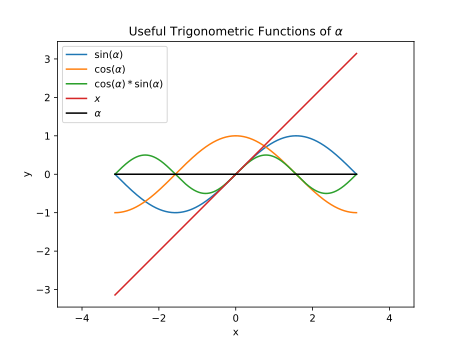
\includegraphics[width=.75\textwidth]{images/plotSinCos}
	\caption{Plot of $\alpha$, $\sin\alpha$, $\cos\alpha$ and $\sin\alpha*\cos\alpha$}
	\label{fig:plotSinCos}
\end{figure}

This shows that, in the neighborhood of $(\alpha, \theta)=(0, 0)$, the distance error $e$ converges at a rate of $\text{exp}(-\gamma t)$ while the angle errors converge at a rate of $\text{exp}(-\sigma t)$ where $-\sigma$ is the real part of the dominant pole of the linear system $A$ in (\ref{eq:lyapunovLinearSystem}) which can be found from the eigenvalues of $A$. The reason that the errors converge at those rates is that, for the distance error, $e=\text{exp}(-\gamma t)$ is a solution to the equation $\dot{e}=-\gamma e$ since 
\begin{align*}
\tfrac{d}{dt}e=\tfrac{d}{dt}\text{exp}(-\gamma t) = -\gamma \text{exp}(-\gamma t)=-\gamma e.
\end{align*}
Similarly, the behavior of the angle errors is related to the matrix $A$ and nonsingular matrices can be factored into the form $A=S\Lambda S^{-1}$ where $S$ contains the eigenvectors of $A$ and $\Lambda$ is a diagonal matrix containing the eigenvalues of $A$. The solution to the differential equation is
\begin{align*}
\left[\begin{array}{c} \dot{\alpha} \\ \dot{\theta} \end{array}\right] = \text{exp}(At)=\text{exp}(S\Lambda S^{-1}t)=S\text{exp}(\Lambda t)S^{-1}
\end{align*}
and $\dot{\alpha}$ has the solution $\alpha=\text{exp}(\lambda_\alpha t)$ and $\dot{\theta}$ has the solution $\theta=\text{exp}(\lambda_\theta t)$.

Three reasonable design considerations in selecting the gains are:
\begin{itemize}
\item limit the maximum linear velocity,
\item find critically damped gains,
\item have angle errors converge before distance error.
\end{itemize}
Limiting the maximum linear velocity has been discussed already and involves the selection of $\gamma$. The damping of the system $A$ is determined by
\begin{align*}
\zeta = \frac{\lambda_\alpha(A)}{\lambda_\theta(A)}
\end{align*}
and the gains are critically damped when $\zeta = 1 \Rightarrow \lambda_\alpha(A)=\lambda_\theta(A)=\lambda$ so that both angle errors $\alpha$ and $\theta$ are converging to zero at the same rate. When the system is critically damped the angle errors will converge before the distance error if $\sigma>\gamma$ since that means the rate of convergence for the angle errors is greater than the rate of convergence for the distance error. In the case where the $A$ matrix is overdamped $\zeta > 1 \Rightarrow \lambda_\alpha(A) > \lambda_\theta(A)$ then $\alpha$ will converge to zero before $\theta$ and conversely when $A$ is underdamped $\zeta < 1$ and $\theta$ converges before $\alpha$.

By selecting the gains to satisfy the design considerations above the robot will align itself with the goal heading before arriving at the goal point and will smoothly decrease its linear velocity as it approaches the goal point. One alternative occurs when the distance error converges before the angle errors, $\gamma>\sigma$, and the robot will get to the goal point and then finish aligning with the goal heading which has several problems: (i) the robot does not look as intelligent since the trajectory does not appear to be as "natural" as the way a human would drive and (ii) rotating in place is typically a much more difficult maneuver for tracked robots to perform and increases the fatigue on the treads compared to turning while driving forward. The other alternative is that one angle error will converge before the other and this can lead to oscillations in heading since the two angle errors are coupled.

To deterministically discover gains that will satisfy the properties discussed two conditions must be met:
\begin{itemize}
\item $\zeta = 1$
\item $\sigma > \gamma$
\end{itemize}
For $\zeta=1$ it is necessary to first determine the eigenvalues of $A$.
\begin{align*}
&(A-\lambda I) = \left[\begin{array}{c c} -k-\lambda & -h\gamma \\ \gamma & -\lambda\end{array}\right] = 0 \\
\Rightarrow &(-k-\lambda)(-\lambda)+h\gamma^2 = 0 \\
\Rightarrow &\lambda^2 + k\lambda + h\gamma^2 = 0 \\
\Rightarrow &\lambda = \frac{-k\pm\sqrt{k^2-4h\gamma^2}}{2}
\end{align*}
For $\lambda_\alpha(A)=\lambda_\theta(A)$ the term inside the square root must be equal to zero resulting in
\begin{align*}
&k^2 - 4h\gamma^2 = 0 \\
\Rightarrow &k = \sqrt{4h\gamma^2} = 2\gamma\sqrt{h}
\end{align*}
To find $\sigma>\gamma$ constrained by $k=2\gamma\sqrt{h}$ it is necessary to have
\begin{align*}
\sigma &= -\lambda = \tfrac{k}{2} > \gamma \\
\Rightarrow k &> 2\gamma
\end{align*}
The two equations can be combined to find $h$ such that
\begin{align*}
k &= 2\gamma\sqrt{h} > 2\gamma \\
\Rightarrow h &> 1
\end{align*}

Using this method any two gains can be selected and the third gain can be found which satisfies the above properties. For example, setting $\gamma=0.2$ to limit the maximum linear velocity and $h=1.1$ to keep it small but greater than one leads to $k=2\gamma\sqrt{h}=0.42$. From this it can be seen that $\lambda_\alpha(A) = \lambda_\theta(A) = 0.21 \Rightarrow \zeta = 1$ so the system $A$ is critically damped and $\sigma = 0.21>0.2=\gamma$ so that the angle errors will converge before the distance error.

\subsection{Model Based Driving Mode}
\label{sec:drivingMode}
The parking mode described above can be extended such that the control law will cause the robot to drive through intermediate waypoints on a route rather than stop at each waypoint.

*** In driving mode the determination of whether the robot is within a capture radius of the current waypoint so that the next waypoint becomes the current target has to be modified. One way to do this is to artificially move the current waypoint position by $W_x += \cos(\psi)$ and $W_y += \sin(\psi)$. If this is not done then the robot will overshoot the waypoint because the error distance has been increased and the angle errors will increase causing the robot to slow down and go back to the original waypoint position. It looks stupid. ***

*** Talk about how gains with $e$ converging before $\alpha$ before $\theta$ could be better in driving mode. ***

The model based controller developed in this Chapter along with the analysis of selecting appropriate gains replaces the original PID controller when answering the question "How do I get there?".

\chapter{Results}
\label{ch:results}
The Kalman filter and controls algorithms discussed in this thesis were implemented in software on a Packbot and run in an open field with an uneven surface consisting of dirt, gravel and asphalt as seen in Figure \ref{fig:resultsTestArea}. This testing area is difficult for the robots to navigate because pitch, roll and elevation have significant changes and the loose dirt and gravel can cause the tracks to slip leading to erroneous encoder data. The environment in addition to routes that force the robot to change linear and angular velocities excites all the modes of the system model as well as some effects, such as track slip, which are not modeled at all and rigorously tests the estimation and control algorithms.

\begin{figure}[ht!]
	\centering
	\includegraphics[width=.75\textwidth]{images/flightFieldTestArea}
	\caption{Robot Test Area}
	\label{fig:resultsTestArea}
\end{figure}

\section{Kalman Filter Results}
\label{sec:kfResults}
In Chapter \ref{ch:estimation} several aspects of the Kalman filter were modified with the goal of improving robot state estimation. Two metrics have been used to quantify the difference in performance of the Kalman filter after having made changes to the algorithm. Those metrics are the RMS error over the entire course and the amount of error in the position estimate before and after the robot runs a route where the percentage is the position error divided by the total amount of distance traveled over the route. Also included is the total distance traveled during the run that the data was logged. The different changes that were tested were the baseline case, fixing the Kalman filter implementation bugs described in Chapter \ref{sec:kfBugs}, hand tuning the Kalman filter noise models and finally using noise models learned from the training algorithm from Chapter \ref{sec:kftrainingparams}. The results for Kalman filter performance are shown in Table \ref{tab:resultsKF}.

% Note for data sources: baseline is 20010107_1037, fixes is 20100107_1411, hand tuned is 20100107_1415, trained is 20100107_1905.
\begin{table}[ht!]
\caption{Kalman Filter Performance}
\small
\centering
\begin{tabular}{@{}lllr@{}} \toprule
Stage      & RMS Error (m)  & Return Error (\%) & Distance Traveled (m) \\ \midrule
Baseline   & 10.62          & 1.51              & 224.22 \\
Fix Bugs   & 4.38           & 0.79              & 182.70 \\
Hand Tuned & 4.87           & 1.32              & 184.09 \\
Trained    & 3.64           & 0.99              & 332.62 \\ \bottomrule
\end{tabular}
\label{tab:resultsKF}
\end{table}

The most significant improvement came from fixing the bugs in the Kalman filter code. Using the training algorithm to tune the parameters in the noise models showed a marked improvement over the hand tuned case and was also better on average than the case where the bugs were fixed. Although the trained noise models case has a slightly greater error in the difference between starting and stopping positions that run was much greater in total distance traveled and a return error of $0.99\%$ over a $332m$ run is more than sufficient to perform retrotraverse in most environments where the robots are used.

\subsection{Kalman Filter Effects on Controller}
Early on during testing, before the bugs were discovered and fixed in the Kalman filter, several runs were logged that show how estimation errors can affect the model based and PID controllers. In this section the data was collected before the bugs in the Kalman filter were fixed (Chapter \ref{sec:kfBugs}) but training of the noise models was used (Chapter \ref{sec:kftrainingparams}). The results are interesting because they show that the previous performance of the PID controller could break down and become unusable as well as because it shows that the training algorithm can improve a filter with equations that are not optimal. The results show that not only is the Kalman filter performance better after using the training algorithm but it can also be seen that the model based controller has much better performance when there are simulated obstacles along the route.

In Figures \ref{fig:kfResults1} - \ref{fig:kfResults4} the same route was driven and the waypoints making up the route are shown on the overhead images. The red line is the Kalman filter position esimate, the blue line is raw GPS measurements and the green line is DPGS measurements.

The results of using the model based controller with original noise models is shown in Figure \ref{fig:kfResults1}. It can be seen that going from waypoint $4$ to waypoint $5$ the Kalman filter started to diverge significantly from the GPS measurements and the filter estimate snaps back to line up with the GPS measurements.

\begin{figure}[ht!]
	\centering
	\includegraphics[width=.75\textwidth]{images/GE/20101203_1551_kf_lyapOrigQR}
	\caption{Model Based Controller with Original Noise Models}
	\label{fig:kfResults1}
\end{figure}

Running the model based controller with learned noise models resulted in the positions shown in Figure \ref{fig:kfResults2}. Here it can be seen that the Kalman filter position estimate is much closer to the GPS measurements for the entire route and that in certain places, such as near waypoint $4$ and between waypoint $6$ and waypoint $7$ the Kalman filter is able to remove discontinuities in the GPS position. Also, in the section of the route with waypoints close to each other to simulate navigation around obstacles the model based controller is able to drive through the waypoints.

\begin{figure}[ht!]
	\centering
	\includegraphics[width=.75\textwidth]{images/GE/20101203_1545_kf_lyapNewQR}
	\caption{Model Based Controller with Learned Noise Models}
	\label{fig:kfResults2}
\end{figure}

The PID controller with original noise models is shown in Figure \ref{fig:kfResults3}. Similar results are seen in regards to the Kalman filter position estimate snapping to the GPS measurements when significant divergence occurs between wayoint $2$ and waypoint $3$. The PID controller has trouble in the section of the route between waypoint $6$ and waypoint $12$ where the waypoints were set up close together to simulate obstacle along the route. In this section of the route the Kalman filter yaw estimate becomes very poor as the robot was driving in circles trying to reach the waypoints and as a result the Kalman filter position estimate diverges and would have snapped back to the GPS measurement if the route were not finished at waypoint $14$.

\begin{figure}[ht!]
	\centering
	\includegraphics[width=.75\textwidth]{images/GE/20101203_1755_kf_pidOrigQR}
	\caption{PID Controller with Original Noise Models}
	\label{fig:kfResults3}
\end{figure}

The PID controller with learned noise models has similar trouble navigating the waypoints that are close together as seen in Figure \ref{fig:kfResults4}. However, with the learned noise models the Kalman filter position estimate stays much closer to the GPS measurements even when the robot is driving in circles. The improved position estimate is also indicative of an improved yaw estimate from the Kalman filter.

\begin{figure}[ht!]
	\centering
	\includegraphics[width=.75\textwidth]{images/GE/20101203_1751_kf_pidNewQR}
	\caption{PID Controller with Learned Noise Models}
	\label{fig:kfResults4}
\end{figure}

\section{Model Based Controller Results}
\label{sec:lyapunovResults}
The linear and angular velocity outputs that were the result of running a simple route with the PID controller are shown in Figure \ref{fig:pidOutput}. This compares to the outputs of the model based controller shown in Figure \ref{fig:mbOutput} where it can be seen that the angular velocity is smooth and the linear velocity drives much faster, using $100\%$ effort at times but smoothly decelerating as waypoints are reached. The linear velocity output does not go to zero until the final waypoint is reached as a consequence of the moving target frame described in Chapter \ref{sec:drivingMode}. The errors for the model based controller are shown in Figure \ref{fig:mbErrors} which shows that $e$, $\alpha$ and $\theta$ decrease linearly at the rate given by the gain $\gamma$ and the eigenvalues of the matrix $A$ composed of the gains $h$ and $k$.

\begin{figure}[ht!]
	\centering
	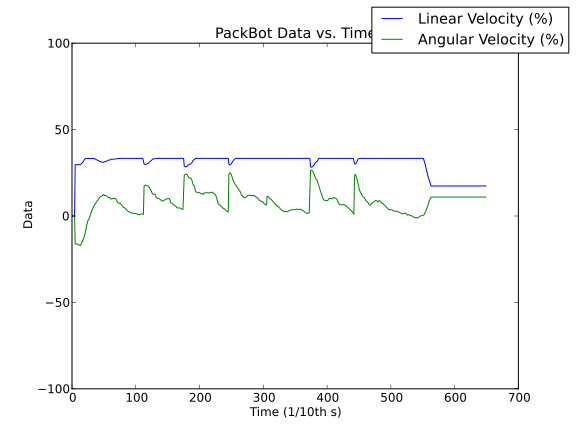
\includegraphics[width=.5\textwidth]{images/pbtx/20110109_1815_pbtx_simpleDrivePID}
	\caption{Typical PID Controller Velocity Output}
	\label{fig:pidOutput}
\end{figure}

\begin{figure}[ht!]
	\centering
	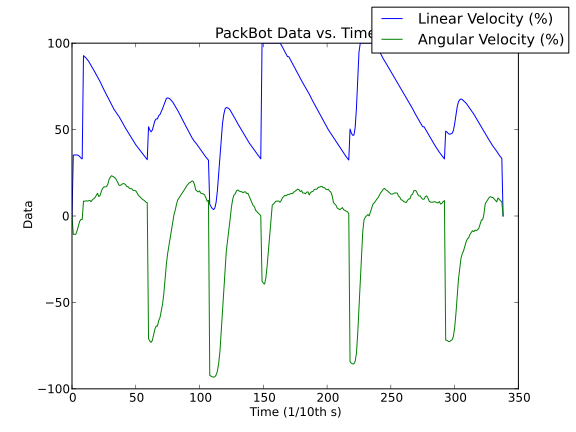
\includegraphics[width=.5\textwidth]{images/pbtx/20110113_1451_pbtx_simpleDrive}
	\caption{Typical Model Based Controller Velocity Output}
	\label{fig:mbOutput}
\end{figure}

\begin{figure}[ht!]
	\centering
	\includegraphics[width=.5\textwidth]{images/pbtx/20110113_1451_pbtx_simpleDriveErrors}
	\caption{Model Based Controller Errors}
	\label{fig:mbErrors}
\end{figure}

\subsection{Controller Comparison}
\label{sec:controllerComparison}
For both PID (Chapter \ref{sec:pid}, Table \ref{tab:PIDGainEffects}) and the model based controller (Chapter \ref{sec:lyapunovTrajectoryConvergence}) gains have to be selected, the difference being that stability is the goal when selecting PID gains whereas stability is guaranteed with the model based controller. More advanced behaviors such as three point turns are a consequence of the control law in (\ref{eq:lyapunovControlLaw}) derived using a kinematic model of the robot. The other very large difference between the controllers is that a table of gains must be tuned for the PID controller to work at varying linear velocities but the model based controller works very well at different linear and angular velocities. Also, when properties of the robot such as mass are changed by using different payloads for the system the entire table of PID gains must be retuned while, at most, one set of gains must be retuned for the model based controller. This last benefit of the model based controller makes it very appealing to use in fielded systems since it reduces the amount of maintenance and effort required to keep the robot in optimal working condition. The model based controller will also allow for improved navigation performance near obstacles which leads directly to improved autonomy for the robot. The local path planner is much simpler with the model based controller since it simply requires moving the target frame based on the calculated errors whereas the PID controller uses an entirely new algorithm that is not a normal part of the control algorithm to set the carrot following mode \cite{Hogg02}.

Many different controller configurations are possible based on varying the gains used and the calculation of the desired heading at waypoints. The tested configurations included:
\begin{enumerate}
\item PID with best available gains,
\item Fuzzy logic with best available rules,
\item Model based with $\theta^\star$ set as angle from current waypoint to next waypoint with gains set to minimize $e$ before angle errors ($\gamma = 0.25$, $h = 0.33$, $k = 0.30$),
\item Model based with $\theta^\star$ set as angle from previous waypoint to current waypoint with gains set to minimize $e$ before angle errors ($\gamma = 0.25$, $h = 0.33$, $k = 0.30$),
\item Model based with $\theta^\star$ set as angle from current waypoint to next waypoint with gains set to minimize angle errors before $e$ ($\gamma = 0.25$, $h = 1.1$, $k = 2\gamma\sqrt{h}$),
\item Model based with $\theta^\star$ set as angle from previous waypoint to current waypoint with gains set to minimize angle errors before $e$ ($\gamma = 0.25$, $h = 1.1$, $k = 2\gamma\sqrt{h}$),
\end{enumerate}
Note that in all cases for the model based controller the desired goal heading $\theta^\star$ for the final waypoint was set to be the angle from the previous waypoint to the last waypoint.

Each controller configuration was run on several courses that test specific behaviors such as
\begin{itemize}
\item allowing for maximum velocities to be sustained with large amounts of open space on the route by having long path segments shown in Figure \ref{fig:routeLong}, with $\lambda = 0.001$, $\epsilon = 2.0$, $R_{\text{cap}} = 1.0$ and there are $13$ waypoints covering a total of $90.73 m$ with an average distance between them of $7.56 m$,
\begin{figure}[ht!]
	\centering
	\includegraphics[width=.5\textwidth]{images/GE/GELongSegmentsRoute2}
	\caption{Route with Long Path Segments}
	\label{fig:routeLong}
\end{figure}
\item short path segments between waypoints to simulate obstacles along the route shown in Figure \ref{fig:routeShort}, with $\lambda = 0.001$, $\epsilon = 1.0$, $R_{\text{cap}} = 0.2$ and there are $27$ waypoints covering a total of $43.18 m$ with an average distance between them of $1.66 m$,
\begin{figure}[ht!]
	\centering
	\includegraphics[width=.5\textwidth]{images/GE/GEShortSegmentsRoute2}
	\caption{Route with Short Path Segments}
	\label{fig:routeShort}
\end{figure}
\item a mixture of long and short path segments shown in Figure \ref{fig:routeMixed}, with $\lambda = 0.001$, $\epsilon = 1.5$, $R_{\text{cap}} = 0.5$ and there are $13$ covering a total of $70.87 m$ waypoints with an average distance between them of $5.45 m$.
\begin{figure}[ht!]
	\centering
	\includegraphics[width=.5\textwidth]{images/GE/GEMixedSegmentsRoute2}
	\caption{Route with Mixed Length Path Segments}
	\label{fig:routeMixed}
\end{figure}
\end{itemize}
The variable $R_{\text{cap}}$ is the capture radius for each waypoint which is used to determine when the robot is close enough to the current waypoint that the next waypoint should be set as the current target.

The results using the different setups described are shown for the different routes in Tables \ref{tab:resultsControllersOpenSpace} - \ref{tab:resultsControllersMixed} where the metrics used to compare the controller performance are
\begin{itemize}
\item the time required to complete the course,
\item the average cross track (XT) error during the course to show whether the robot followed a straight line between waypoints which is important when obstacles are in the area and not important when large amounts of open space are available for navigation (although some operators become nervous when the robot trajectory has large curvature and deviates from a straight line path even if open space is available),
\item the maximum velocity achieved by the robot during the course,
\item the number of times that the robot stops where a stop is defined as the robot having a velocity that drops below a small velocity,
\item the average error in heading from the desired heading when reaching the waypoints which is not available for the PID or fuzzy logic controllers but does help to differentiate between the model based controllers that have different goal headings and gains,
\item the total effort used by summing the values of linear and angular velocity over an entire run but does not take into account accelerations or the orientation of the robot.
\end{itemize}
For the model based controller in parking mode the same algorithm was run but $\epsilon=0$ was enough to keep the distance error from increasing and $\lambda$ was unused.

\begin{table}[ht!]
\caption{Controller Comparison on Open Space Route}
\small
\centering
\begin{tabular}{@{}llllr@{}} \toprule
Setup & Time (s) & XT (m) & $u_{\text{max}}$ (\%) & Stops \\ \midrule
1     & 82.67    & 0.61   & 33.3                  & 1     \\
2     & 0        & 0      & 0                     & 0     \\
3     & 75.12    & 2.52   & 100.0                 & 3     \\
4     & 71.42    & 2.71   & 100.0                 & 4     \\
5     & 110.09   & 2.42   & 100.0                 & 14    \\
6     & 75.45    & 2.80   & 100.0                 & 5     \\ \bottomrule
\end{tabular}
\label{tab:resultsControllersOpenSpace}
\end{table}

\begin{table}[ht!]
\caption{Controller Comparison on Simulated Obstacle Route}
\small
\centering
\begin{tabular}{@{}llllr@{}} \toprule
Setup & Time (s) & XT (m) & $u_{\text{max}}$ (\%) & Stops \\ \midrule
1     & N/A      & N/A    & N/A                   & N/A   \\
2     & 0        & 0      & 0                     & 0     \\
3     & 134.92   & 0.85   & 42.52                 & 20    \\
4     & 75.92    & 0.94   & 50.86                 & 21    \\
5     & 232.09   & 0.79   & 27.90                 & 31    \\
6     & 75.99    & 0.91   & 49.96                 & 23    \\ \bottomrule
\end{tabular}
\label{tab:resultsControllersObstacles}
\end{table}

\begin{table}[ht!]
\caption{Controller Comparison on Mixed Route}
\small
\centering
\begin{tabular}{@{}llllr@{}} \toprule
Setup & Time (s) & XT (m) & $u_{\text{max}}$ (\%) & Stops \\ \midrule
1     & N/A      & N/A    & N/A                   & N/A   \\
2     & 0        & 0      & 0                     & 0     \\
3     & 103.39   & 2.51   & 100.0                 & 11    \\
4     & 76.91    & 2.98   & 100.0                 & 12    \\
5     & 164.65   & 2.34   & 100.0                 & 22    \\
6     & 83.84    & 2.87   & 100.0                 & 12    \\ \bottomrule
\end{tabular}
\label{tab:resultsControllersMixed}
\end{table}

The PID controller only worked well on the route with long path segments. For the short and mixed path segment routes it actually became sad to watch and the tests were aborted because the robot was just spinning in circles and running the batteries down, similar to what was seen in Figure \ref{fig:kfResults4}.

All of the model based controllers are fairly similar. However, it can be seen that Setup $3$ consistently has longer run times but smaller cross track errors. This indicates that during those runs the robot was on the line between the previous and current waypoints with a heading towards the waypoint but that the robot slowed down at each of the waypoints because the angle errors were larger than in other runs. For all three routes each configuration of the model based controller exhibits an inverse relationship between cross track error and time taken to complete the route. The best setup for the most common scenarios that SSCPAC robots will encounter is likely to be either Setup $4$ or Setup $6$ where the robot drives fast and stays fairly close the straight line path between waypoints. Those two setups have the desired goal heading, $\theta^\star$, set to be the angle from the previous waypoint to the current waypoint which has more to do with the robot staying on the line between waypoints than do the gains.

%\chapter{Future Work}
\label{ch:futurework}

\begin{enumerate}
\item Use the results from this work to make retrotraverse work better. One way this can be accomplished is that obstacles should be easier to avoid since the robot position is more accurate so following a previously navigated path after some time has passed should result in less drift so previously avoided static obstacles will be closer to where they were before. Additionally, a control law that works at varying speeds (like Lyapunov, unlike PID that had to be tuned with different gains for different speeds) will make navigation around obstacles smoother and faster.
\item Work on a planner that can automatically tune the gains for the Lyapunov controller based on the environment of the robot. For example, if there are no nearby obstacles then let the path curvature be large. If the environment is cluttered then force the path curvature to be much smaller.
\item Use the learning algorithm for indoor robots as there is no reason why a robot needs to have GPS to benefit from using the DGPS system for training the $Q$ and $R$ matrices in the EKF. A test area would need to be set up outdoors so that DGPS can be used and the normal sensors also work by bouncing off walls and what not but the DGPS ground truth position can be converted to the local coordinate system and used to generate an error metric for the EKF position output.
\item Add a high quality IMU that serves as ground truth for Euler angles to the DGPS system so that the training algorithm attempts to minimize the errors between Euler angles in addition to position.
\item Characterize individual IMUs better since that is a large source of error.
\item Say I want to implement the more advanced work done by \cite{Lapierre06} and \cite{Gulati08} to improve the performance of the model-based controller.
\end{enumerate}

\chapter{Conclusion}
\label{ch:conclusion}
*** Summarize the results here. ***
% \appendix % Use \appendix for single, \appendices for multiple
% \include{chapters/sourceCode}
% \chapter{List of Acronyms}
\label{ch:acronyms}
*** Put a list of acronyms here. ***


% Bibliography.
\bibliographystyle{these}
% \bibliographystyle{plain}
\bibliography{mybib}

\end{document}
